\documentclass{article}
\usepackage{graphicx} % Required for inserting Images_Ayoub
\usepackage[french]{babel}
\usepackage{multirow}
\usepackage[utf8]{inputenc}
\usepackage[a4paper,margin=0.5in]{geometry}
\usepackage[T1]{fontenc}
\usepackage{amsmath}
\usepackage{amsthm}
\usepackage{amsfonts}
\usepackage{amsmath}
\usepackage{amssymb}
\usepackage{adjustbox}
\usepackage{listings}
\usepackage{xcolor} % pour définir des couleurs custom
\usepackage[colorlinks=true, linkcolor=blue, urlcolor=blue, citecolor=blue]{hyperref}

% Définir une couleur de fond gris clair
\definecolor{lightgray}{gray}{0.95}
\usepackage{array}
\usepackage{siunitx} % Pour la notation scientifique
\usepackage{graphicx}
\usepackage{subcaption} % Pour les sous-figures
\usepackage{booktabs} % Pour de meilleurs tableaux
\usepackage{subcaption}  % Nécessaire pour les sous-figures
\usepackage{tikz}
\usetikzlibrary{3d,perspective,quotes,angles}
\pgfdeclarelayer{background}
\pgfsetlayers{background,main}
\usepackage{tikz}
\usetikzlibrary{shapes.geometric, arrows.meta, positioning}
\usepackage{tikz}
\usepackage{tikz-3dplot}
\usetikzlibrary{arrows.meta, backgrounds, calc, positioning, decorations.pathreplacing, angles, quotes}
\usepackage{algorithm}
\usepackage{algpseudocode}
% Définir l'entrée dans la table des matières et la commande subsubsubsection
\makeatletter
% Créer un nouveau compteur pour subsubsubsection
\newcounter{subsubsubsection}[subsubsection]
% Format du numéro : ex. 1.2.3.4
\renewcommand\thesubsubsubsection{\thesubsubsection.\@arabic\c@subsubsubsection}
% Définition de la commande subsubsubsection
\newcommand\subsubsubsection{\@startsection{subsubsubsection}{4}{\z@}%
    {-1.5ex \@plus -0.2ex \@minus -0.2ex}% Espace avant
    {0.5ex \@plus 0.2ex}% Espace après
    {\normalfont\normalsize\bfseries}}% Style de la police
% Commande pour le marquage dans le texte (optionnel)
\newcommand{\subsubsubsectionmark}[1]{}
% Ajouter subsubsubsection à la table des matières
\makeatother

% Définir les commandes tocloft pour subsubsubsection
\makeatletter
% Définir l'entrée dans la table des matières
\newcommand{\l@subsubsubsection}{\@dottedtocline{4}{7em}{4em}}
% Définir les commandes pour l'indentation et la largeur du numéro
\newcommand{\cftsubsubsubsecindent}{7em}
\newcommand{\cftsubsubsubsecnumwidth}{4em}
\makeatother

% Configurer la profondeur de la table des matières
\setcounter{tocdepth}{4}
\setcounter{secnumdepth}{4}

\begin{document}

\begin{titlepage}
\begin{center}
    
\includegraphics[width=0.3\linewidth]{Images_Ayoub/Logo/Logo.png}
\end{center}
    \centering
    \vspace*{3in} % Ajuste la hauteur pour centrer verticalement
    \Huge \textbf{Report : Molecular energy prediction} \\[1cm] % Titre
    \Large {Par Ayoub CHOUKRI et Axel OLOUGOUNA} \\ % Auteu
    \Large \date{March 2025} % Date
    \vfill
\end{titlepage}

\newpage

\tableofcontents

\newpage

\section*{Introduction}

The Molecular Energy Prediction project, undertaken as part of ModIA 2025, aims to develop a unified model for predicting the atomization energy \( E(\mathbf{r}) \) of small organic molecules based on their 3D atomic positions \( \mathbf{r} \) and additional atomic properties. Leveraging a subset of the QM7-X dataset, which includes 4739 molecular structures, this study addresses a high-dimensional regression problem while adhering to critical symmetry constraints—namely translational, rotational, and permutational invariance. The challenge lies in designing a model that remains robust under these transformations, a key aspect explored through the application of 3D scattering methods inspired by the Kymatio tutorial, alongside other innovative approaches. Additionally, we explored a second approach involving a data transformation to ensure invariance under rotation, translation, and permutation, followed by the application of transformers to enhance prediction accuracy. This report outlines our methodology, from data preprocessing to model evaluation, and discusses the potential implications and future directions of our findings in the context of quantum chemistry regression. \newline



\section{QM7-X Dataset}

The QM7-X dataset is a collection of 4739 small organic molecules, each represented by a set of atomic positions and their corresponding atomization energies. The dataset is designed to facilitate the development and evaluation of machine learning models for predicting molecular properties based on geometric and electronic structure information. Each molecule in the dataset is characterized by:  \newline

The QM7-X dataset consists of files in the \texttt{xyz} format, a standard in computational chemistry for representing the three-dimensional structure of molecules. Each \texttt{xyz} file describes a molecule by listing its atoms, their types (chemical symbols), and their Cartesian coordinates $(x, y, z)$ in space. This format enables precise visualization and analysis of molecular geometry. \newline

Below is an example visualization of a molecule from the dataset:
\begin{center}
    \begin{minipage}{0.95\linewidth}
      \centering
      \setlength{\fboxsep}{0pt} % Supprime l'espacement entre l'image et le cadre
      \fbox{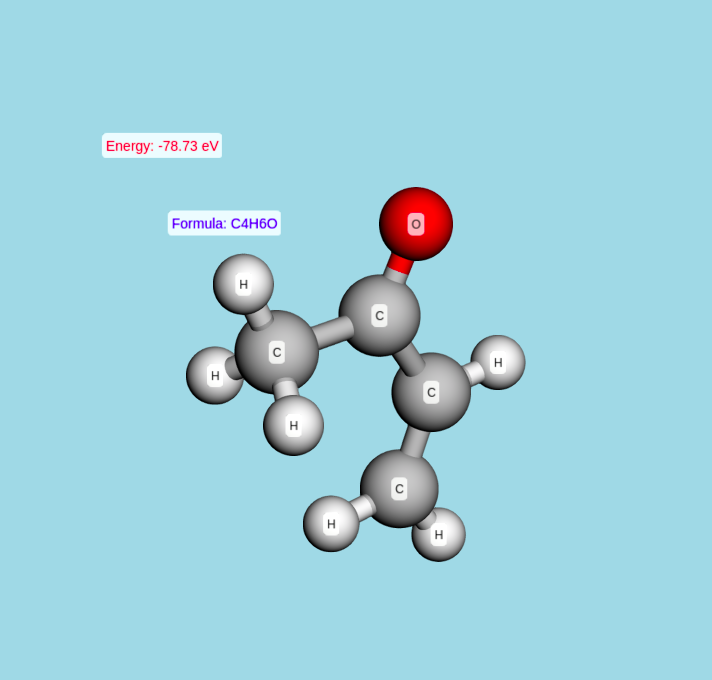
\includegraphics[width=0.8\linewidth]{Images_Ayoub/Dataset/Molecule/image.png}} % Cadre autour de l'image
      \captionof{figure}{Exemple de molécule extraite du dataset QM7-X, visualisée à partir de ses coordonnées \texttt{xyz}.}
      \label{fig:xyz_molecule_example}
    \end{minipage}
\end{center}
\section{First approach : 3D Wavelet Scattering for Molecular Energy Prediction}

The main idea of this approach is to use 3D wavelet scattering to extract features from the 3D atomic positions of molecules. The scattering transform is a powerful tool for capturing local and global geometric features while ensuring invariance to translation, rotation, and permutation of atoms. This method allows us to create a robust representation of molecular structures that can be used for regression tasks, such as predicting molecular energies. \newline

Moreover, the 3D wavelet scattering transform naturally produces features that are invariant under translation, rotation, and permutation of atoms. This invariance is crucial for molecular data, as the physical properties of a molecule do not depend on its absolute position, orientation, or the ordering of its atoms. By leveraging these invariances, the model can focus on learning the intrinsic properties of molecular structures without being affected by irrelevant transformations. \newline


\subsection{3D Wavelets: Mathematical Formulation and Properties}

The 3D wavelet scattering transform relies on a family of 3D wavelets, which are localized functions designed to analyze spatial variations in electron densities at multiple scales and orientations. In this context, the wavelets are constructed to ensure translation, rotation, and permutation invariance, making them well-suited for molecular data.

\subsubsection{Definition of 3D Wavelets}

A 3D wavelet $\psi_{l,k}(\mathbf{r})$ is defined as a function on $\mathbb{R}^3$ that is localized in both space and frequency.  \newline

More specifically, The Morlet wavelet is defined as:

\[
\psi_{j,\ell}(u) = 2^{-2j} \psi(2^{-j} r_{\theta_\ell} u)
\]

for \( u \in \mathbb{R}^2 \), where \(\theta_\ell = \frac{\ell \pi}{L}\) with \( 0 \leq \ell < 2L \). This wavelet incorporates a scaling factor \( 2^{-2j} \) and a rotation \( r_{\theta_\ell} \), making it suitable for applications requiring specific frequency and orientation analysis. \newline




The family $\{\psi_{l,k}\}$ spans multiple scales $l$ and orientations $k$, enabling multi-resolution analysis of 3D signals.

\subsubsection{Properties of 3D Wavelets}

\begin{itemize}
  \item \textbf{Localization}: 3D wavelets are localized in both space and frequency, allowing them to capture local geometric features of molecular densities.
  \item \textbf{Multi-scale Analysis}: By varying the scale parameter $j$, wavelets can analyze features at different spatial resolutions, from fine atomic details to global molecular shapes.
  \item \textbf{Directional Sensitivity}: The use of harmonics $\psi_{j,l}$ provides sensitivity to angular variations, enabling the capture of directional patterns in the data.
  \item \textbf{Invariance}: When combined with appropriate integration and modulus operations in the scattering transform, the resulting features are invariant to translation, rotation, and permutation of atoms. \newline
\end{itemize}







3D wavelets provide a mathematically rigorous and physically meaningful way to analyze molecular electron densities. Their multi-scale, multi-orientation structure, combined with the invariance properties of the scattering transform, makes them a powerful tool for extracting features relevant to molecular energy prediction. \newline


To apply the Wavelet Scattering transform, a data preprocessing step is required. This will be detailed in the following subsection.


\subsubsection{Visualisation of an example of 2D Wavelet Scattering Transform}

\begin{figure}[H]
    \centering
    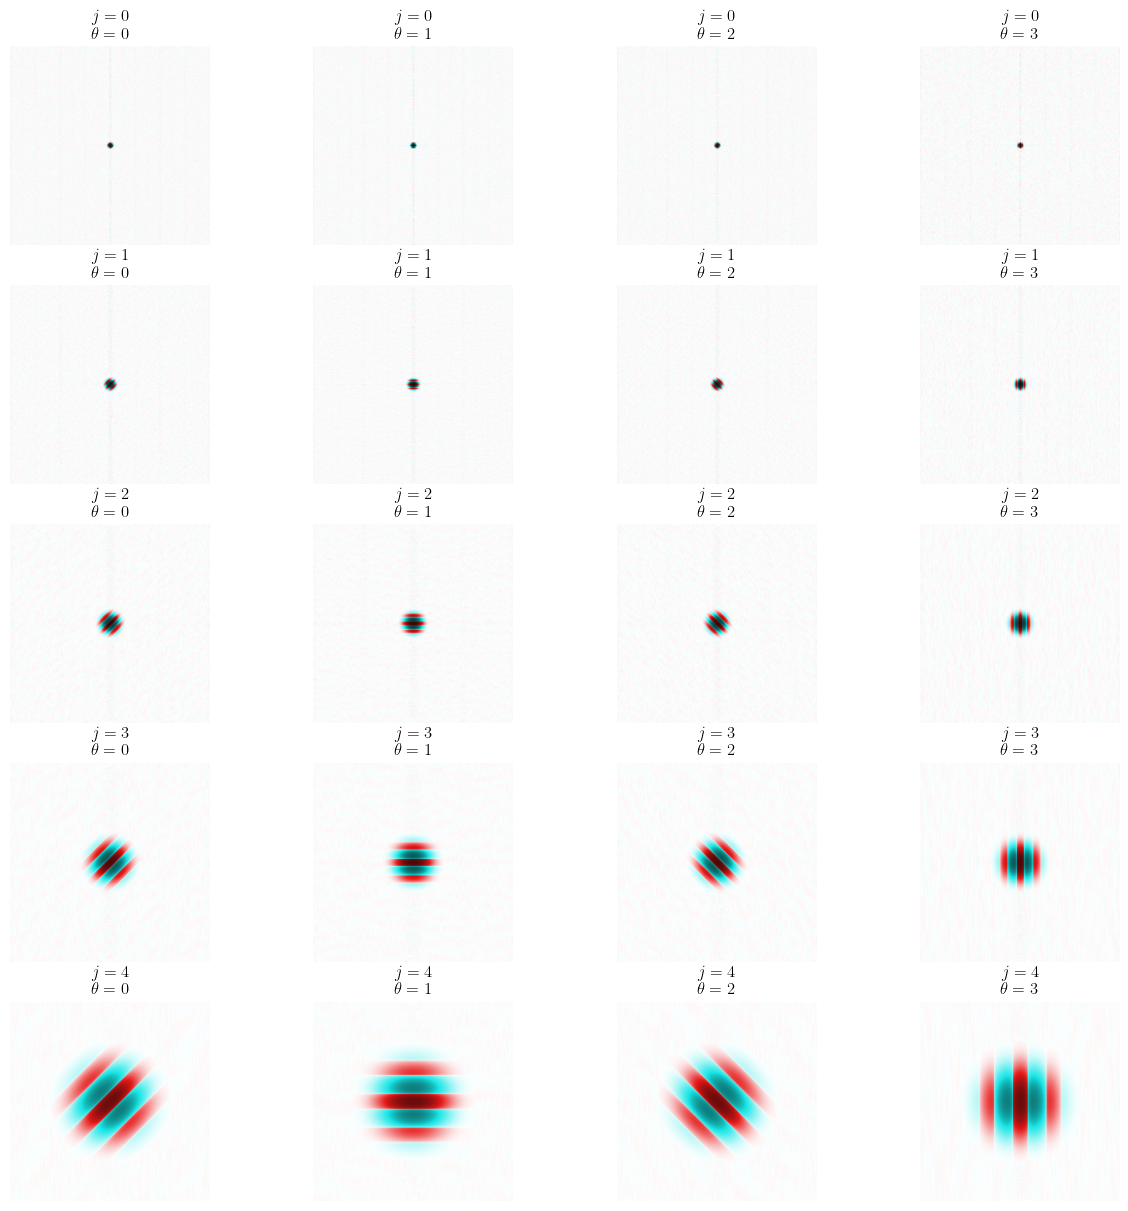
\includegraphics[width=0.8\textwidth]{Images_Ayoub/Wavelets/Image.png}
    \caption{Example of 2D Wavelet Scattering Transform}
    \label{fig:2D_wavelet_scattering}
\end{figure}

\subsection{Data Preprocessing and Transformation}

The 3D wavelet scattering transform for molecular energy prediction requires preprocessing raw molecular data into a standardized format suitable for computing electron density representations and extracting invariant scattering features. Consider a molecule $M$ with $A$ atoms. The dataset for molecule $M$ contains the following components:

\begin{itemize}
    \item A list of atomic symbols: $[S_1, S_2, \ldots, S_A]$
    \vspace{0.2cm}
    \item 3D positions, represented as a matrix of coordinates: $[\mathbf{r}_1, \mathbf{r}_2, \ldots, \mathbf{r}_A]$, where $\mathbf{r}_i = [x_i, y_i, z_i] \in \mathbb{R}^3$
    \vspace{0.2cm}
    \item Molecular energy: $E \in \mathbb{R}$
\end{itemize}

\vspace{0.2cm}

The molecular energy $E$ serves as the target for regression. This preprocessing converts the data into fixed-size numerical representations to ensure numerical stability and consistency across molecules with varying numbers of atoms. The resulting data enables the generation of electron density functions and the extraction of features invariant to translation, rotation, and permutation of atoms, essential for accurate regression of molecular properties such as energy. \newline

The preprocessing pipeline involves mapping atomic types to nuclear charges, estimating valence charges, scaling atomic positions, padding data to a uniform size, constructing electron density functions, and computing scattering features. These steps are described below with their mathematical formulations. \newline

\subsubsection{Nuclear Charges}

The molecular data includes atomic symbols, 3D coordinates, and an energy value. Atomic symbols are mapped to their nuclear charges (atomic numbers, $Z$) using a predefined mapping:

\[
\text{mapping} = \{ \text{H}: 1, \text{C}: 6, \text{N}: 7, \text{O}: 8, \text{S}: 16, \text{Cl}: 17 \}
\]

The nuclear charges are represented as a vector:

\[
\mathbf{q} = [Z_1, Z_2, \ldots, Z_A], \quad Z_i \in \{1, 6, 7, 8, 16, 17\}
\]


\subsubsection{Valence Charge Estimation}

To distinguish between core and valence electron contributions, valence charges are estimated based on nuclear charges using a periodic table-based heuristic:

\[
v_i =
\begin{cases}
Z_i & \text{if } Z_i \leq 2 \\
Z_i - 2 & \text{if } 2 < Z_i \leq 10 \\
Z_i - 10 & \text{if } 10 < Z_i \leq 18
\end{cases}
\]

This yields a valence charge vector:

\[
\mathbf{v} = [v_1, v_2, \ldots, v_A]
\]

For instance, carbon ($Z = 6$) has $v = 4$ valence electrons, and sulfur ($Z = 16$) has $v = 6$. These charges enable the construction of separate density functions for valence and core electrons.

\subsubsection{Position Scaling}

To ensure consistent density overlap and numerical stability in the scattering transform, atomic positions are scaled based on the minimum interatomic distance:

\[
d_{ij} = |\mathbf{r}_i - \mathbf{r}_j|, \quad d_{\text{min}} = \min_{i \neq j} d_{ij}
\]

A scaling factor $\delta$ is computed using a Gaussian width $\sigma = 2.0$ and an overlap parameter $\epsilon = 0.1$:

\[
\delta = \sigma \sqrt{-8 \ln(\epsilon)}
\]

Positions are scaled as:

\[
\mathbf{r}_i' = \mathbf{r}_i \cdot \frac{\delta}{d_{\text{min}}}
\]

This normalization aligns the minimum interatomic distance with $\sigma$, ensuring that Gaussian functions used in density computations have controlled overlap, with $\exp\left(-\frac{d_{\text{min}}^2}{2\sigma^2}\right)$ decaying to a value related to $\epsilon$.

\subsubsection{Data Padding}

To support batch processing, nuclear charges, valence charges, and positions are padded with zeros to a fixed size, defined by the maximum number of atoms ($A_{\text{max}} = 23$):

\[
\mathbf{q}' = [\mathbf{q}, 0, \ldots, 0] \in \mathbb{R}^{A_{\text{max}}}, \quad \mathbf{v}' = [\mathbf{v}, 0, \ldots, 0] \in \mathbb{R}^{A_{\text{max}}}, \quad \mathbf{R}' = [\mathbf{R}, \mathbf{0}, \ldots, \mathbf{0}] \in \mathbb{R}^{A_{\text{max}} \times 3}
\]

This ensures uniform tensor dimensions across all molecules.

\subsection{Scattering Transform and Feature Extraction}
\subsubsection{Electron Density Construction}

Electron density functions are constructed on a 3D spatial grid $\mathbf{r} \in \mathbb{R}^3$ as weighted sums of Gaussian functions. The full electron density is:

\[
\rho_{\text{full}}(\mathbf{r}) = \sum_{i=1}^A Z_i \exp\left(-\frac{|\mathbf{r} - \mathbf{r}_i'|^2}{2\sigma^2}\right)
\]

The valence electron density is:

\[
\rho_{\text{val}}(\mathbf{r}) = \sum_{i=1}^A v_i \exp\left(-\frac{|\mathbf{r} - \mathbf{r}_i'|^2}{2\sigma^2}\right)
\]

The core electron density is:

\[
\rho_{\text{core}}(\mathbf{r}) = \rho_{\text{full}}(\mathbf{r}) - \rho_{\text{val}}(\mathbf{r}) = \sum_{i=1}^A (Z_i - v_i) \exp\left(-\frac{|\mathbf{r} - \mathbf{r}_i'|^2}{2\sigma^2}\right)
\]

These density functions are discretized on a 3D grid for numerical processing.

\subsubsection{Scattering Feature Extraction}

The wavelet scattering transform extracts features from electron density functions that are invariant to translation, rotation, and permutation of atoms. These features are derived by computing zeroth-order integrals and higher-order scattering coefficients, which capture global and local structural properties of the molecule for regression tasks such as energy prediction.

\subsubsubsection{Computing Zeroth-Order Coefficients}

A set of integral powers is defined as $\mathbf{p} = \{p_1, p_2, \ldots\}$, where $p_i \in \mathbb{R}$ represents the powers for moment calculations. For each electron density function $\rho(\mathbf{r})$ (e.g., full, valence, or core density), the zeroth-order coefficients are computed as the integrals of the module of the density raised to the power $p_i$:

\[
I_{p_i} = \int |\rho(\mathbf{r})|^{p_i} \, d\mathbf{r}, \quad p_i \in \mathbf{p}
\]

For $p_i = 1$, the integral represents the total absolute charge:

\[
I_1 = \int |\rho(\mathbf{r})| \, d\mathbf{r}
\]

These coefficients provide global descriptors of the density, capturing its magnitude and distribution, which are used as invariant features in the scattering transform. Notably, these integrals are invariant under translation: shifting all atomic positions by a constant vector does not change the value of the integrals, since the density function is simply shifted in space and the integration domain covers all of \(\mathbb{R}^3\). \newline


\textbf{Proof of Translation Invariance}

Let us prove that the zeroth-order coefficients
\[
I_{p} = \int_{\mathbb{R}^3} |\rho(\mathbf{r})|^{p} \, d\mathbf{r}
\]
are invariant under translation of all atomic positions.

Suppose we translate all atomic positions by a fixed vector \(\mathbf{a} \in \mathbb{R}^3\). The new density is
\[
\rho'(\mathbf{r}) = \rho(\mathbf{r} - \mathbf{a})
\]
The corresponding integral becomes
\[
I_{p}' = \int_{\mathbb{R}^3} |\rho'(\mathbf{r})|^{p} \, d\mathbf{r} = \int_{\mathbb{R}^3} |\rho(\mathbf{r} - \mathbf{a})|^{p} \, d\mathbf{r}
\]
Let us change variables: set \(\mathbf{u} = \mathbf{r} - \mathbf{a}\), so \(d\mathbf{u} = d\mathbf{r}\). Then
\[
I_{p}' = \int_{\mathbb{R}^3} |\rho(\mathbf{u})|^{p} \, d\mathbf{u} = I_{p}
\]
Thus, the integral is unchanged by translation. Therefore, the zeroth-order coefficients are invariant under translation.



\subsubsubsection{Computing Higher-Order Scattering Coefficients}

The First order coefficients are computed by convolving the electron density with a set of wavelet filters, followed by computing the module and integrating over the 3D space : 

$$
S_1(l) =\frac{1}{2L} \sum_{k=0}^{2L-1} \int |\rho * \psi_{l,k}(\mathbf{r})| \, d\mathbf{r}
$$



The second order coefficients are computed by convolving the first order coefficients with a set of wavelet filters, followed by computing the module and integrating over the 3D space :

$$
S_2(l,\theta_1,\theta_2) = \frac{1}{2L} \sum_{k=0}^{2L} \int | \rho * \psi_{l,\theta_1 - k }| * \psi_{l,\theta_2 - k }(\mathbf{r})|^p \, d\mathbf{r}
$$


\subsubsubsection{Feature Vector Construction}

The feature vector for each molecule is constructed by concatenating the zeroth-order and higher-order scattering coefficients. This results in a comprehensive representation that captures both global and local structural information : 

\[
\mathbf{S} = \begin{bmatrix}
S_0(\rho_{\text{full}}) \\
S_0(\rho_{\text{val}}) \\
S_0(\rho_{\text{core}}) \\
S_1(\rho_{\text{full}}) \\
S_1(\rho_{\text{val}}) \\
S_1(\rho_{\text{core}}) \\
S_2(\rho_{\text{full}}) \\
S_2(\rho_{\text{val}}) \\
S_2(\rho_{\text{core}})
\end{bmatrix}
\]



\subsection{Coulomb Matrix for Molecular Energy Prediction}

The Coulomb Matrix approach provides a compact representation of molecular structures for predicting atomization energy by encoding pairwise electrostatic interactions between atoms. To ensure invariance under translation, rotation, and permutation, we extract the sorted eigenvalues of the Coulomb Matrix, which serve as the primary feature vector for regression. This eigenvalue-based representation captures the essential chemical and geometric properties of the molecule while satisfying the required symmetry constraints. Padding is applied to the eigenvalue vector to handle molecules with varying numbers of atoms, ensuring compatibility with regression models such as kernel ridge regression or neural networks. Below, we detail the construction of the Coulomb Matrix, its invariance properties, and the feature extraction process.

\subsubsection{Construction of the Coulomb Matrix}

For a molecule \( M \) with \( A \) atoms, the Coulomb Matrix \( \mathbf{C} \) is a symmetric \( A \times A \) matrix that quantifies electrostatic interactions. Given the nuclear charges \( \mathbf{q} = [Z_1, Z_2, \ldots, Z_A] \) (as defined in Section 1.1.1) and the scaled atomic positions \( \mathbf{R}' = [\mathbf{r}_1', \mathbf{r}_2', \ldots, \mathbf{r}_A'] \in \mathbb{R}^{A \times 3} \) (from Section 1.1.3), the matrix elements are defined as:

\[
C_{ij} =
\begin{cases} 
0.5 Z_i^{2.4} & \text{if } i = j, \\
\frac{Z_i Z_j}{|\mathbf{r}_i' - \mathbf{r}_j'|} & \text{if } i \neq j
\end{cases}
\]

The diagonal elements \( C_{ii} = 0.5 Z_i^{2.4} \) approximate the self-energy of atom \( i \), with the exponent 2.4 empirically chosen to reflect atomic energy scaling. The off-diagonal elements \( C_{ij} \) represent the Coulomb repulsion between atoms \( i \) and \( j \), scaled by their interatomic distance \( |\mathbf{r}_i' - \mathbf{r}_j'| \). The resulting matrix encodes the molecular structure, but its eigenvalues and eigenvectors are extracted to ensure invariance properties.

\subsubsection{Invariance Properties}

The eigenvalue-based representation of the Coulomb Matrix satisfies the symmetry constraints required for molecular energy prediction, namely invariance under translation, rotation, and permutation of atoms. These properties ensure that the feature vector remains consistent regardless of the molecule’s position, orientation, or atom ordering.

\subsubsubsection{Translational Invariance}

The Coulomb Matrix is inherently invariant under translation because it depends only on the relative distances \( |\mathbf{r}_i' - \mathbf{r}_j'| \). If all atomic positions are translated by a constant vector \( \mathbf{a} \in \mathbb{R}^3 \), the new positions become \( \mathbf{r}_i'' = \mathbf{r}_i' + \mathbf{a} \), and the distances remain unchanged:

\[
|\mathbf{r}_i'' - \mathbf{r}_j''| = |(\mathbf{r}_i' + \mathbf{a}) - (\mathbf{r}_j' + \mathbf{a})| = |\mathbf{r}_i' - \mathbf{r}_j'|
\]

Thus, the matrix elements \( C_{ij} \) (both diagonal and off-diagonal) are unaffected, and the eigenvalues of \( \mathbf{C} \), which depend only on the matrix’s structure, remain invariant under translation.

\subsubsubsection{Rotational Invariance}

The eigenvalues of the Coulomb Matrix ensure rotational invariance. A rotation corresponds to applying an orthogonal transformation \( \mathbf{Q} \in \mathbb{R}^{3 \times 3} \) (where \( \mathbf{Q}^T \mathbf{Q} = \mathbf{I} \)) to the atomic positions: \( \mathbf{r}_i'' = \mathbf{Q} \mathbf{r}_i' \). The interatomic distances are preserved:

\[
|\mathbf{r}_i'' - \mathbf{r}_j''| = |\mathbf{Q} \mathbf{r}_i' - \mathbf{Q} \mathbf{r}_j'| = |\mathbf{Q} (\mathbf{r}_i' - \mathbf{r}_j')| = |\mathbf{r}_i' - \mathbf{r}_j'|
\]

While the raw Coulomb Matrix may vary due to atom indexing, its eigenvalues are invariant under similarity transformations, including rotations. Sorting the eigenvalues ensures a consistent representation, making the feature vector rotationally invariant.

\subsubsubsection{Permutational Invariance}

The raw Coulomb Matrix is sensitive to the ordering of atoms, as permuting two atoms \( i \) and \( j \) would swap the corresponding rows and columns of \( \mathbf{C} \). However, the eigenvalues and \textbf{sorted} eigenvectors of \( \mathbf{C} \) are invariant to such permutations, as they depend only on the matrix’s intrinsic properties. By sorting the eigenvalues, we obtain a fixed-size vector that is unaffected by atom reordering, ensuring permutational invariance.

\subsubsection{Data Padding for Uniform Representation}

To accommodate molecules with varying numbers of atoms, the extracted eigenvectors are padded to a fixed length corresponding to the maximum number of atoms, \( A_{\text{max}} = 23 \). For a molecule with \( A \leq A_{\text{max}} \) atoms, the Coulomb Matrix \( \mathbf{C} \in \mathbb{R}^{A \times A} \) has \( A \) eigenvalues \( \lambda = [\lambda_1, \lambda_2, \ldots, \lambda_A] \), sorted in descending order. The padded eigenvalue vector is:

\[
\lambda' = [\lambda_1, \lambda_2, \ldots, \lambda_A, 0, \ldots, 0] \in \mathbb{R}^{A_{\text{max}}}
\]

This ensures uniform input dimensions across all molecules, enabling efficient batch processing in regression models.

\subsubsection{Feature Extraction and Regression}

The sorted and padded eigenvalue vector \( \lambda' \) serves as the feature vector for predicting the atomization energy \( E \). This representation captures the electrostatic and geometric properties of the molecule in a manner that is invariant under translation, rotation, and permutation. The feature vector is input to a regression model, such as kernel ridge regression or a neural network, optimized for the QM7-X dataset (4739 molecules). The Coulomb Matrix eigenvectors approach complements the 3D wavelet scattering transform by providing a simpler representation focused on pairwise interactions. Subsequent sections will evaluate the performance of this approach and explore its integration with scattering-based features to enhance prediction accuracy.


\subsection{Ridge Regression}

\subsubsection{Model Description}

Ridge regression is a linear regression technique that incorporates L2 regularization to prevent overfitting, especially in high-dimensional datasets. The model aims to minimize the following loss function:

\[
\min_{\beta} \; \sum_{i=1}^{N} \left( y_i - \beta^T \mathbf{x}_i \right)^2 + \lambda \|\beta\|_2^2
\]

\subsubsection{Cross Validation}


To optimize the regularization parameter \(\lambda\) in Ridge regression, \(k\)-fold cross-validation is used to select the value of \(\lambda\) that minimizes the model's prediction error on unseen data. The process is described mathematically as follows:

\begin{enumerate}
    \item \textbf{Data Partitioning}: 
    Let the dataset consist of \(N\) samples, denoted as \(\mathcal{D} = \{(\mathbf{x}_i, y_i)\}_{i=1}^N\), where \(\mathbf{x}_i \in \mathbb{R}^p\) is the feature vector and \(y_i \in \mathbb{R}\) is the target value. The dataset is randomly divided into \(k\) disjoint subsets (folds) of approximately equal size, denoted \(\mathcal{D}_1, \mathcal{D}_2, \ldots, \mathcal{D}_k\), such that \(\mathcal{D} = \bigcup_{j=1}^k \mathcal{D}_j\) and \(\mathcal{D}_j \cap \mathcal{D}_l = \emptyset\) for \(j \neq l\). Each fold \(\mathcal{D}_j\) contains roughly \(N/k\) samples.

    \item \textbf{Training and Validation Split}: 
    For each fold \(j = 1, 2, \ldots, k\), define the training set as \(\mathcal{D}_{\text{train}}^{(j)} = \mathcal{D} \setminus \mathcal{D}_j\) (all data except the \(j\)-th fold) and the validation set as \(\mathcal{D}_{\text{val}}^{(j)} = \mathcal{D}_j\). The training set contains approximately \((k-1)N/k\) samples, and the validation set contains \(N/k\) samples.

    \item \textbf{Model Training}: 
    For a fixed value of \(\lambda\), train the Ridge regression model on \(\mathcal{D}_{\text{train}}^{(j)}\) by solving the optimization problem:
    \[
    \hat{\beta}^{(j)}(\lambda) = \arg\min_{\beta} \sum_{(\mathbf{x}_i, y_i) \in \mathcal{D}_{\text{train}}^{(j)}} \left( y_i - \beta^T \mathbf{x}_i \right)^2 + \lambda \|\beta\|_2^2,
    \]
    where \(\hat{\beta}^{(j)}(\lambda) \in \mathbb{R}^p\) is the estimated coefficient vector for the \(j\)-th fold and given \(\lambda\). The closed-form solution is:
    \[
    \hat{\beta}^{(j)}(\lambda) = \left( \mathbf{X}_{\text{train}}^{(j)T} \mathbf{X}_{\text{train}}^{(j)} + \lambda \mathbf{I}_p \right)^{-1} \mathbf{X}_{\text{train}}^{(j)T} \mathbf{y}_{\text{train}}^{(j)},
    \]
    where \(\mathbf{X}_{\text{train}}^{(j)}\) is the design matrix of the training set, \(\mathbf{y}_{\text{train}}^{(j)}\) is the corresponding target vector, and \(\mathbf{I}_p\) is the \(p \times p\) identity matrix.

    \item \textbf{Validation Error Computation}: 
    Using the trained model \(\hat{\beta}^{(j)}(\lambda)\), compute the mean squared error (MSE) on the validation set \(\mathcal{D}_{\text{val}}^{(j)}\):
    \[
    \text{MSE}_{\text{val}}^{(j)}(\lambda) = \frac{1}{|\mathcal{D}_{\text{val}}^{(j)}|} \sum_{(\mathbf{x}_i, y_i) \in \mathcal{D}_{\text{val}}^{(j)}} \left( y_i - \hat{\beta}^{(j)}(\lambda)^T \mathbf{x}_i \right)^2,
    \]
    where \(|\mathcal{D}_{\text{val}}^{(j)}|\) is the number of samples in the validation set (approximately \(N/k\)).

    \item \textbf{Average Validation Error}: 
    Repeat steps 2–4 for each fold \(j = 1, 2, \ldots, k\), and compute the average validation error for the given \(\lambda\):
    \[
    \text{MSE}_{\text{CV}}(\lambda) = \frac{1}{k} \sum_{j=1}^k \text{MSE}_{\text{val}}^{(j)}(\lambda).
    \]

    \item \textbf{Hyperparameter Tuning}: 
    Evaluate \(\text{MSE}_{\text{CV}}(\lambda)\) over a grid of candidate \(\lambda\) values, typically chosen on a logarithmic scale, e.g., \(\lambda \in \{10^{-3}, 10^{-2}, \ldots, 10^3\}\). Select the optimal \(\lambda^*\) that minimizes the cross-validation error:
    \[
    \lambda^* = \arg\min_{\lambda} \text{MSE}_{\text{CV}}(\lambda).
    \]

    \item \textbf{Final Model}: 
    Using the selected \(\lambda^*\), retrain the Ridge regression model on the entire dataset \(\mathcal{D}\) to obtain the final coefficient vector:
    \[
    \hat{\beta}(\lambda^*) = \arg\min_{\beta} \sum_{i=1}^{N} \left( y_i - \beta^T \mathbf{x}_i \right)^2 + \lambda^* \|\beta\|_2^2,
    \]
    where \(\mathbf{X}\) and \(\mathbf{y}\) are the design matrix and target vector for the full dataset.
\end{enumerate}

This \(k\)-fold cross-validation process ensures that the selected \(\lambda^*\) balances the trade-off between model complexity (controlled by \(\lambda \|\beta\|_2^2\)) and predictive accuracy, leading to a model that generalizes well to unseen data.



\subsection{Practical Proof  of Invariance under Translation, Rotation}
To empirically validate the invariance properties of our model, we conducted a series of experiments using the QM7-X dataset. The objective was to demonstrate that the scattering coefficients remain consistent under various transformations, specifically permutation, translation, and rotation of molecular structures. \newline

For each transformation, we selected a molecule and applied the corresponding operation: permuting the order of atoms, translating all atomic coordinates by a random vector, or rotating the entire structure using a random rotation matrix. We then computed the scattering coefficients before and after each transformation and evaluated the maximum relative errors to quantify the invariance. The results showed that the scattering coefficients remain consistent up to numerical precision, with maximum relative errors below a predefined threshold, providing robust evidence of the model's invariance properties. \newline

Since permutation invariance is inherently ensured by the model's design, which processes atoms in a symmetric manner, we focused our empirical validation on rotation and translation invariance, as these transformations are more challenging to enforce and critical for accurate molecular modeling.


\subsubsection{Translation Invariance}

To test the translation invariance of our model, we translated all atomic coordinates of a selected molecule by a randomly chosen vector. We then verified that the predicted energy did not change and that each atomic position was consistently shifted by the same vector. The following report shows the detailed comparison before and after translation, as well as the computed differences.
\begin{figure}[H]
  \centering
  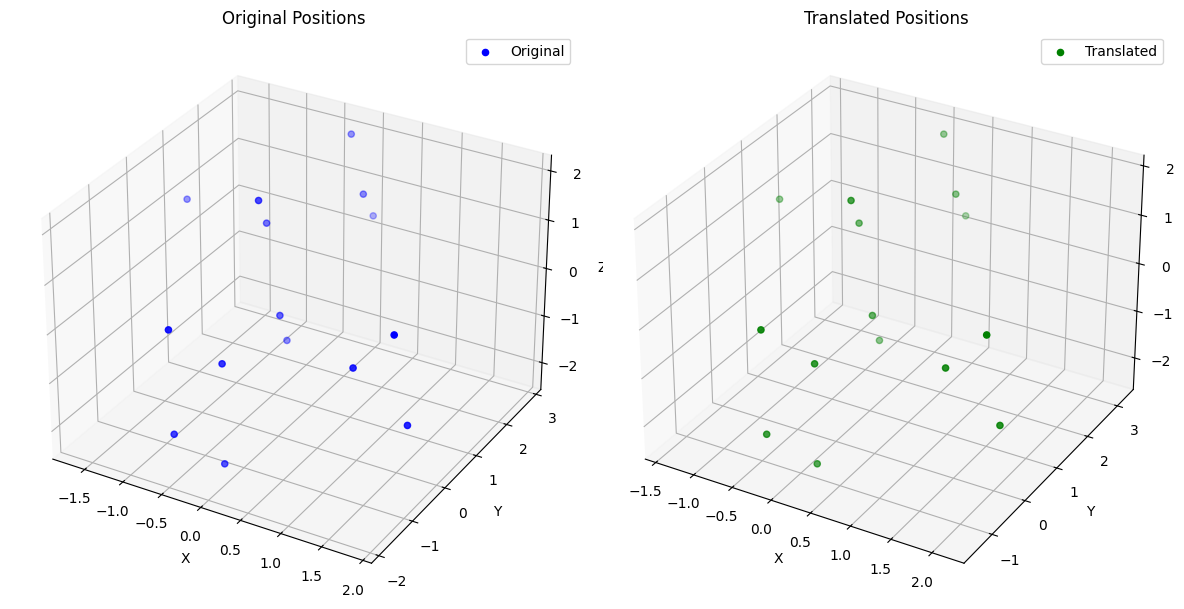
\includegraphics[width=0.85\linewidth]{Images_Ayoub/Invariance/Scattering/Translation.png}
  \caption{Visualization of the molecule before and after a random translation applied during the translation invariance test.}
  \label{fig:translation_invariance_visualization}
\end{figure}

\begin{lstlisting}[
  language={},
  basicstyle=\ttfamily\small,
  backgroundcolor=\color{lightgray},
  frame=single
]
=== Scattering Translation Invariance Test Report (15:36:39 2025-06-29) ===
Molecule ID: 4893

+-------------------------------------+--------------+
|               Metric                |    Value     |
+-------------------------------------+--------------+
|    Max Relative Error (Order 0)     | 7.544136e-07 |
| Max Relative Error (Orders 1 and 2) | 2.031497e-04 |
|          Invariance Check           |     PASS     |
+-------------------------------------+--------------+

Translation Vector:
+------+-----------+
| Axis |   Value   |
+------+-----------+
|  X   |  0.282500 |
|  Y   |  0.386503 |
|  Z   | -0.101358 |
+------+-----------+

Atom Position Comparison (Part 1: Original Positions):
+----+-----------+-----------+-----------+
|    |   X_old   |   Y_old   |   Z_old   |
+----+-----------+-----------+-----------+
| 1  |  0.132120 |  2.237617 |  1.199850 |
| 2  | -0.562639 |  0.959334 |  1.023047 |
| 3  | -0.075889 |  0.232029 | -0.224623 |
| 4  |  1.193155 | -0.598378 | -0.171746 |
| 5  | -0.141514 | -1.263526 | -0.317596 |
| 6  | -0.482658 | -1.871082 | -1.543105 |
| 7  | -0.236380 |  2.738383 |  2.004059 |
| 8  |  0.024724 |  2.821760 |  0.374761 |
| 9  | -1.664761 |  1.097503 |  0.958059 |
| 10 | -0.384184 |  0.334583 |  1.910556 |
| 11 | -0.226950 |  0.780826 | -1.156448 |
| 12 |  1.709371 | -0.664955 |  0.780528 |
| 13 |  1.847253 | -0.560436 | -1.037480 |
| 14 | -0.542706 | -1.830043 |  0.527811 |
| 15 | -0.068618 | -1.389036 | -2.270445 |
+----+-----------+-----------+-----------+

Atom Position Comparison (Part 2: Translated Positions):
+----+-----------+-----------+-----------+
|    |   X_new   |   Y_new   |   Z_new   |
+----+-----------+-----------+-----------+
| 1  |  0.414620 |  2.624120 |  1.098492 |
| 2  | -0.280139 |  1.345837 |  0.921689 |
| 3  |  0.206611 |  0.618532 | -0.325981 |
| 4  |  1.475655 | -0.211875 | -0.273104 |
| 5  |  0.140986 | -0.877023 | -0.418954 |
| 6  | -0.200158 | -1.484579 | -1.644463 |
| 7  |  0.046120 |  3.124886 |  1.902701 |
| 8  |  0.307224 |  3.208263 |  0.273403 |
| 9  | -1.382261 |  1.484006 |  0.856701 |
| 10 | -0.101684 |  0.721086 |  1.809198 |
| 11 |  0.055550 |  1.167329 | -1.257806 |
| 12 |  1.991871 | -0.278452 |  0.679170 |
| 13 |  2.129753 | -0.173933 | -1.138838 |
| 14 | -0.260206 | -1.443540 |  0.426453 |
| 15 |  0.213882 | -1.002533 | -2.371803 |
+----+-----------+-----------+-----------+

Atom Position Comparison (Part 3: Position Differences):
+----+--------+----------+-----------+
|    |   dX   |    dY    |    dZ     |
+----+--------+----------+-----------+
| 1  | 0.2825 | 0.386503 | -0.101358 |
| 2  | 0.2825 | 0.386503 | -0.101358 |
| 3  | 0.2825 | 0.386503 | -0.101358 |
| 4  | 0.2825 | 0.386503 | -0.101358 |
| 5  | 0.2825 | 0.386503 | -0.101358 |
| 6  | 0.2825 | 0.386503 | -0.101358 |
| 7  | 0.2825 | 0.386503 | -0.101358 |
| 8  | 0.2825 | 0.386503 | -0.101358 |
| 9  | 0.2825 | 0.386503 | -0.101358 |
| 10 | 0.2825 | 0.386503 | -0.101358 |
| 11 | 0.2825 | 0.386503 | -0.101358 |
| 12 | 0.2825 | 0.386503 | -0.101358 |
| 13 | 0.2825 | 0.386503 | -0.101358 |
| 14 | 0.2825 | 0.386503 | -0.101358 |
| 15 | 0.2825 | 0.386503 | -0.101358 |
+----+--------+----------+-----------+
\end{lstlisting}


During our experiments, we observed that translation invariance is well maintained when the translation vector applied to the molecule is small. However, when the translation vector becomes very large, this invariance is no longer perfectly verified: The scattering coefficients may change severally with a relative error that can reach up to 50\%.

\subsubsection{Rotation Invariance Test Report}


To assess the rotation invariance of our model, we applied a random rotation defined by a given angle and axis to the atomic coordinates of a selected molecule. We then verified that the predicted energy remained unchanged and inspected how each atom's position transformed under this rotation.


\begin{figure}[H]
  \centering
  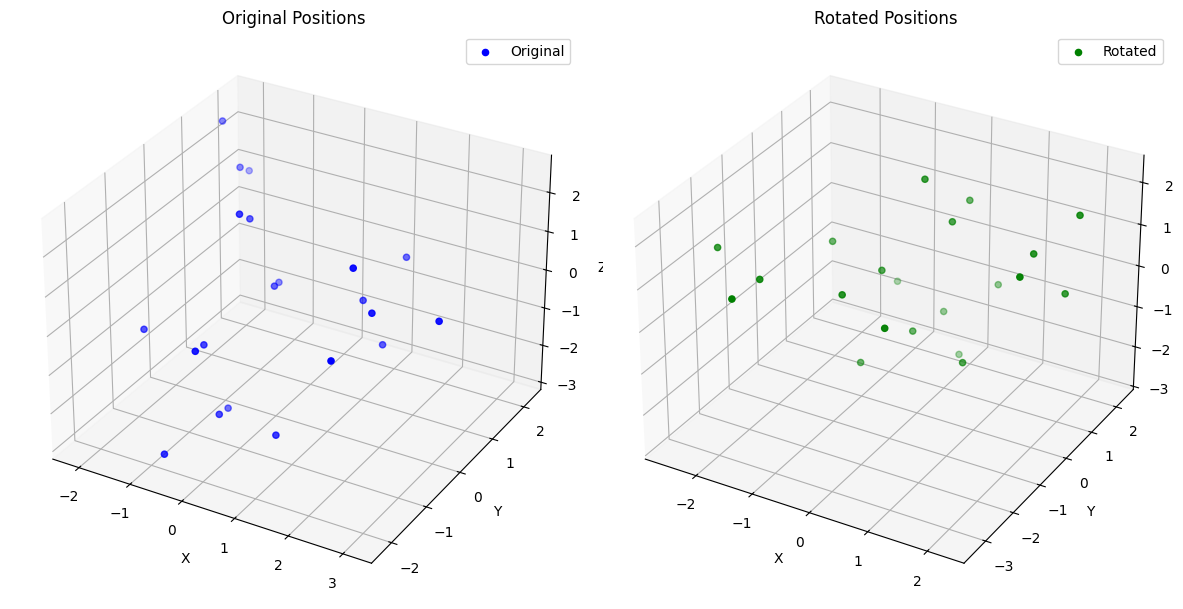
\includegraphics[width=0.9\linewidth]{Images_Ayoub/Invariance/Scattering/Rotation.png}
  \caption{Visualization of the molecule before and after a random rotation applied during the rotation invariance test.}
  \label{fig:rotation_invariance_visualization}
\end{figure}





\begin{lstlisting}[
  language={},
  basicstyle=\ttfamily\small,
  backgroundcolor=\color{lightgray},
  frame=single
]
=== Scattering Rotation Invariance Test Report (16:37:54 2025-06-29) ===
Molecule ID: 4517

+-------------------------------------+--------------+
|               Metric                |    Value     |
+-------------------------------------+--------------+
|    Max Relative Error (Order 0)     | 3.987890e-07 |
| Max Relative Error (Orders 1 and 2) | 1.347913e-02 |
|          Invariance Check           |     FAIL     |
+-------------------------------------+--------------+

Rotation Details:
+-------------------+-----------------------------------+
|     Parameter     |               Value               |
+-------------------+-----------------------------------+
| Point A (X, Y, Z) | (-0.493018, -0.096519, -0.265246) |
| Point B (X, Y, Z) |  (0.318869, -0.162669, 0.327524)  |
|  Angle (degrees)  |             90.000000             |
+-------------------+-----------------------------------+

Atom Pairwise Distances (Original, Rotated, Difference):
+-----------+--------------+--------------+-----------+
| Atom Pair | Old Distance | New Distance |   Diff    |
+-----------+--------------+--------------+-----------+
|    1-2    |   1.523262   |   1.523262   | -0.000000 |
|    1-3    |   2.576324   |   2.576324   | -0.000000 |
|    1-4    |   3.888297   |   3.888296   | -0.000001 |
|    1-5    |   4.867879   |   4.867878   | -0.000001 |
|    1-6    |   3.122869   |   3.122867   | -0.000001 |
|    1-7    |   3.724528   |   3.724528   | -0.000001 |
|    1-8    |   1.088217   |   1.088217   |  0.000000 |
|    1-9    |   1.087772   |   1.087773   |  0.000000 |
|   1-10    |   1.088328   |   1.088328   | -0.000000 |
|   1-11    |   2.153358   |   2.153357   | -0.000000 |
|   1-12    |   2.145956   |   2.145956   | -0.000001 |
|   1-13    |   2.779874   |   2.779874   | -0.000000 |
|   1-14    |   4.296271   |   4.296271   | -0.000000 |
|   1-15    |   4.954390   |   4.954389   | -0.000001 |
|   1-16    |   5.829531   |   5.829530   | -0.000001 |
|   1-17    |   4.107547   |   4.107546   | -0.000001 |
|   1-18    |   2.819258   |   2.819258   | -0.000000 |
|   1-19    |   4.397757   |   4.397756   | -0.000001 |
|   1-20    |   4.504501   |   4.504500   | -0.000001 |
|   1-21    |   3.249571   |   3.249569   | -0.000001 |
|    2-3    |   1.550019   |   1.550018   | -0.000000 |
|    2-4    |   2.509113   |   2.509113   | -0.000001 |
|    2-5    |   3.566796   |   3.566795   | -0.000001 |
|    2-6    |   2.591876   |   2.591875   | -0.000001 |
|    2-7    |   3.122441   |   3.122441   | -0.000001 |
|    2-8    |   2.159688   |   2.159688   | -0.000000 |
|    2-9    |   2.172762   |   2.172762   | -0.000000 |
|   2-10    |   2.168685   |   2.168684   | -0.000000 |
|   2-11    |   1.094815   |   1.094814   | -0.000000 |
|   2-12    |   1.095032   |   1.095032   |  0.000000 |
|   2-13    |   2.157826   |   2.157826   |  0.000000 |
|   2-14    |   2.837977   |   2.837977   | -0.000000 |
|   2-15    |   3.876318   |   3.876318   | -0.000000 |
|   2-16    |   4.441562   |   4.441562   | -0.000000 |
|   2-17    |   3.515658   |   3.515657   | -0.000001 |
|   2-18    |   2.863140   |   2.863139   | -0.000001 |
|   2-19    |   3.459102   |   3.459101   | -0.000001 |
|   2-20    |   4.124307   |   4.124305   | -0.000001 |
|   2-21    |   2.834137   |   2.834135   | -0.000001 |
|    3-4    |   1.515414   |   1.515414   | -0.000001 |
|    3-5    |   2.520776   |   2.520775   | -0.000001 |
|    3-6    |   1.552744   |   1.552743   | -0.000001 |
|    3-7    |   2.596967   |   2.596967   | -0.000001 |
|    3-8    |   3.512940   |   3.512940   | -0.000000 |
|    3-9    |   2.881716   |   2.881716   | -0.000000 |
|   3-10    |   2.811878   |   2.811878   | -0.000000 |
|   3-11    |   2.178075   |   2.178075   | -0.000001 |
|   3-12    |   2.159759   |   2.159759   | -0.000000 |
|   3-13    |   1.102028   |   1.102029   |  0.000000 |
|   3-14    |   2.226342   |   2.226342   | -0.000000 |
|   3-15    |   2.774894   |   2.774894   | -0.000000 |
|   3-16    |   3.508509   |   3.508509   | -0.000000 |
|   3-17    |   2.161437   |   2.161436   | -0.000000 |
|   3-18    |   2.168704   |   2.168704   | -0.000001 |
|   3-19    |   2.857854   |   2.857853   | -0.000001 |
|   3-20    |   3.528043   |   3.528042   | -0.000001 |
|   3-21    |   2.889687   |   2.889686   | -0.000001 |
|    4-5    |   1.333011   |   1.333011   |  0.000000 |
|    4-6    |   2.529318   |   2.529316   | -0.000001 |
|    4-7    |   3.143170   |   3.143169   | -0.000001 |
|    4-8    |   4.662206   |   4.662205   | -0.000001 |
|    4-9    |   4.280233   |   4.280233   | -0.000001 |
|   4-10    |   4.179781   |   4.179780   | -0.000001 |
|   4-11    |   2.764041   |   2.764040   | -0.000001 |
|   4-12    |   2.671971   |   2.671971   | -0.000000 |
|   4-13    |   2.130980   |   2.130980   | -0.000000 |
|   4-14    |   1.090644   |   1.090643   | -0.000000 |
|   4-15    |   2.112862   |   2.112863   |  0.000000 |
|   4-16    |   2.110194   |   2.110195   |  0.000001 |
|   4-17    |   2.716497   |   2.716496   | -0.000001 |
|   4-18    |   3.459476   |   3.459475   | -0.000001 |
|   4-19    |   2.840253   |   2.840252   | -0.000001 |
|   4-20    |   4.094895   |   4.094893   | -0.000002 |
|   4-21    |   3.592679   |   3.592678   | -0.000001 |
|    5-6    |   3.551620   |   3.551619   | -0.000001 |
|    5-7    |   4.351624   |   4.351624   | -0.000001 |
|    5-8    |   5.635719   |   5.635718   | -0.000001 |
|    5-9    |   5.369979   |   5.369978   | -0.000001 |
|   5-10    |   4.931872   |   4.931871   | -0.000001 |
|   5-11    |   3.983576   |   3.983575   | -0.000001 |
|   5-12    |   3.440934   |   3.440934   | -0.000000 |
|   5-13    |   2.608715   |   2.608715   | -0.000001 |
|   5-14    |   2.094144   |   2.094144   | -0.000001 |
|   5-15    |   1.084222   |   1.084222   | -0.000000 |
|   5-16    |   1.083521   |   1.083522   |  0.000001 |
|   5-17    |   3.422997   |   3.422996   | -0.000001 |
|   5-18    |   4.409233   |   4.409231   | -0.000001 |
|   5-19    |   3.997127   |   3.997127   | -0.000000 |
|   5-20    |   5.209329   |   5.209327   | -0.000001 |
|   5-21    |   4.899267   |   4.899266   | -0.000001 |
|    6-7    |   1.523480   |   1.523480   |  0.000000 |
|    6-8    |   4.131090   |   4.131089   | -0.000001 |
|    6-9    |   2.846194   |   2.846193   | -0.000001 |
|   6-10    |   3.440593   |   3.440592   | -0.000001 |
|   6-11    |   2.857931   |   2.857930   | -0.000001 |
|   6-12    |   3.516484   |   3.516483   | -0.000001 |
|   6-13    |   2.146992   |   2.146991   | -0.000001 |
|   6-14    |   2.905500   |   2.905499   | -0.000000 |
|   6-15    |   3.826982   |   3.826982   | -0.000001 |
|   6-16    |   4.440128   |   4.440128   | -0.000000 |
|   6-17    |   1.095065   |   1.095065   |  0.000000 |
|   6-18    |   1.095233   |   1.095233   | -0.000001 |
|   6-19    |   2.172161   |   2.172161   |  0.000000 |
|   6-20    |   2.158297   |   2.158297   |  0.000000 |
|   6-21    |   2.171734   |   2.171734   | -0.000000 |
|    7-8    |   4.517355   |   4.517355   | -0.000001 |
|    7-9    |   3.253782   |   3.253782   | -0.000001 |
|   7-10    |   4.382263   |   4.382263   | -0.000001 |
|   7-11    |   2.813682   |   2.813681   | -0.000001 |
|   7-12    |   4.107793   |   4.107793   | -0.000001 |
|   7-13    |   3.501050   |   3.501050   | -0.000000 |
|   7-14    |   2.959193   |   2.959193   | -0.000000 |
|   7-15    |   4.914407   |   4.914407   | -0.000000 |
|   7-16    |   5.025961   |   5.025961   | -0.000000 |
|   7-17    |   2.147666   |   2.147666   | -0.000000 |
|   7-18    |   2.148122   |   2.148122   | -0.000000 |
|   7-19    |   1.087879   |   1.087878   | -0.000000 |
|   7-20    |   1.088225   |   1.088224   | -0.000001 |
|   7-21    |   1.087907   |   1.087907   |  0.000000 |
|    8-9    |   1.757520   |   1.757520   |  0.000000 |
|   8-10    |   1.759272   |   1.759272   |  0.000000 |
|   8-11    |   2.498094   |   2.498094   | -0.000000 |
|   8-12    |   2.449769   |   2.449768   | -0.000000 |
|   8-13    |   3.754442   |   3.754443   |  0.000000 |
|   8-14    |   4.947237   |   4.947237   | -0.000000 |
|   8-15    |   5.765704   |   5.765704   | -0.000000 |
|   8-16    |   6.530206   |   6.530206   | -0.000000 |
|   8-17    |   5.150768   |   5.150767   | -0.000001 |
|   8-18    |   3.850365   |   3.850365   | -0.000000 |
|   8-19    |   5.128877   |   5.128876   | -0.000001 |
|   8-20    |   5.301355   |   5.301354   | -0.000001 |
|   8-21    |   3.848000   |   3.847998   | -0.000001 |
|   9-10    |   1.759064   |   1.759064   |  0.000000 |
|   9-11    |   2.500040   |   2.500040   | -0.000000 |
|   9-12    |   3.062045   |   3.062045   | -0.000000 |
|   9-13    |   3.199299   |   3.199299   |  0.000000 |
|   9-14    |   4.595120   |   4.595120   |  0.000000 |
|   9-15    |   5.503840   |   5.503840   | -0.000000 |
|   9-16    |   6.337414   |   6.337414   | -0.000000 |
|   9-17    |   3.861511   |   3.861511   | -0.000000 |
|   9-18    |   2.308213   |   2.308213   | -0.000000 |
|   9-19    |   4.115063   |   4.115062   | -0.000001 |
|   9-20    |   3.836601   |   3.836600   | -0.000001 |
|   9-21    |   2.718293   |   2.718292   | -0.000001 |
|   10-11   |   3.066228   |   3.066227   | -0.000001 |
|   10-12   |   2.525872   |   2.525872   | -0.000000 |
|   10-13   |   2.569226   |   2.569226   | -0.000000 |
|   10-14   |   4.812961   |   4.812961   | -0.000000 |
|   10-15   |   4.777225   |   4.777225   | -0.000000 |
|   10-16   |   5.958333   |   5.958333   | -0.000000 |
|   10-17   |   4.252621   |   4.252621   | -0.000000 |
|   10-18   |   2.985569   |   2.985569   | -0.000000 |
|   10-19   |   5.085732   |   5.085731   | -0.000001 |
|   10-20   |   5.099535   |   5.099534   | -0.000001 |
|   10-21   |   4.100287   |   4.100285   | -0.000001 |
|   11-12   |   1.750234   |   1.750234   | -0.000000 |
|   11-13   |   3.067437   |   3.067436   | -0.000000 |
|   11-14   |   2.653163   |   2.653163   | -0.000000 |
|   11-15   |   4.531109   |   4.531108   | -0.000001 |
|   11-16   |   4.694916   |   4.694915   | -0.000000 |
|   11-17   |   3.835201   |   3.835200   | -0.000001 |
|   11-18   |   3.272830   |   3.272829   | -0.000001 |
|   11-19   |   2.998976   |   2.998975   | -0.000001 |
|   11-20   |   3.839782   |   3.839780   | -0.000001 |
|   11-21   |   2.290713   |   2.290712   | -0.000001 |
|   12-13   |   2.488562   |   2.488562   |  0.000000 |
|   12-14   |   3.056290   |   3.056290   |  0.000000 |
|   12-15   |   3.693783   |   3.693783   | -0.000000 |
|   12-16   |   4.228607   |   4.228607   | -0.000000 |
|   12-17   |   4.307301   |   4.307301   | -0.000000 |
|   12-18   |   3.841865   |   3.841864   | -0.000001 |
|   12-19   |   4.273393   |   4.273392   | -0.000001 |
|   12-20   |   5.146436   |   5.146435   | -0.000001 |
|   12-21   |   3.847931   |   3.847930   | -0.000001 |
|   13-14   |   3.094658   |   3.094658   | -0.000000 |
|   13-15   |   2.403515   |   2.403515   | -0.000000 |
|   13-16   |   3.690052   |   3.690052   | -0.000000 |
|   13-17   |   2.457797   |   2.457797   | -0.000000 |
|   13-18   |   2.411612   |   2.411612   | -0.000000 |
|   13-19   |   3.852627   |   3.852627   | -0.000000 |
|   13-20   |   4.296555   |   4.296554   | -0.000001 |
|   13-21   |   3.840621   |   3.840620   | -0.000001 |
|   14-15   |   3.071768   |   3.071768   | -0.000001 |
|   14-16   |   2.428796   |   2.428795   | -0.000000 |
|   14-17   |   3.182439   |   3.182438   | -0.000000 |
|   14-18   |   3.923269   |   3.923269   | -0.000000 |
|   14-19   |   2.345232   |   2.345233   |  0.000000 |
|   14-20   |   3.923520   |   3.923519   | -0.000001 |
|   14-21   |   3.323941   |   3.323941   |  0.000000 |
|   15-16   |   1.849668   |   1.849668   | -0.000000 |
|   15-17   |   3.605362   |   3.605362   |  0.000000 |
|   15-18   |   4.492378   |   4.492377   | -0.000001 |
|   15-19   |   4.748731   |   4.748731   |  0.000000 |
|   15-20   |   5.714065   |   5.714064   | -0.000001 |
|   15-21   |   5.477686   |   5.477685   | -0.000001 |
|   16-17   |   4.239633   |   4.239633   | -0.000000 |
|   16-18   |   5.376087   |   5.376087   | -0.000001 |
|   16-19   |   4.468378   |   4.468379   |  0.000000 |
|   16-20   |   5.854508   |   5.854508   | -0.000001 |
|   16-21   |   5.591726   |   5.591726   | -0.000000 |
|   17-18   |   1.750543   |   1.750543   | -0.000000 |
|   17-19   |   2.523240   |   2.523239   | -0.000000 |
|   17-20   |   2.457991   |   2.457990   | -0.000001 |
|   17-21   |   3.063096   |   3.063095   | -0.000001 |
|   18-19   |   3.064718   |   3.064717   | -0.000001 |
|   18-20   |   2.480216   |   2.480216   | -0.000000 |
|   18-21   |   2.500271   |   2.500270   | -0.000001 |
|   19-20   |   1.758044   |   1.758043   | -0.000001 |
|   19-21   |   1.759435   |   1.759435   | -0.000000 |
|   20-21   |   1.757155   |   1.757155   | -0.000000 |
+-----------+--------------+--------------+-----------+
\end{lstlisting}
Although the invariance test does not pass for the rotation case (as indicated by the "FAIL" status), it is important to note that the relative error remains quite low. This suggests that, in practice, the model's features are nearly invariant under rotation, with only minor numerical discrepancies.

\subsection{Application and Results}
\subsubsection{CV Fold Losses}

For each value of the regularization parameter \(\alpha\) (or \(\lambda\)), we compute the mean of the mean squared errors (MSE) obtained across the different folds of cross-validation. Mathematically, for each \(\alpha\), the average MSE is given by:
\[
\overline{\text{MSE}}(\alpha) = \frac{1}{k} \sum_{j=1}^k \text{MSE}_{\text{val}}^{(j)}(\alpha)
\]
where \(k\) is the number of cross-validation folds and \(\text{MSE}_{\text{val}}^{(j)}(\alpha)\) is the error on fold \(j\) for parameter \(\alpha\). We then plot the curve \(\overline{\text{MSE}}(\alpha)\) as a function of \(\alpha\) to identify the optimal value that minimizes the validation error.


\begin{figure}[H]
  \centering
  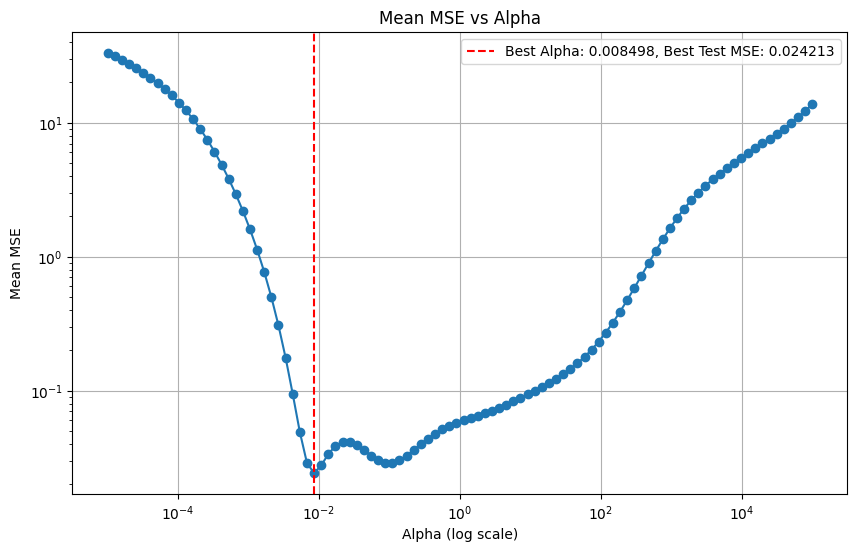
\includegraphics[width=0.8\linewidth]{Images_Ayoub/Training/Scattering/CV/Losses/Loss.png}
  \caption{Curve of the mean cross-validation MSE (\(\overline{\text{MSE}}(\alpha)\)) as a function of the regularization parameter \(\alpha\) for Ridge regression. The minimum of the curve indicates the optimal value of \(\alpha\) selected for the final model.}
  \label{fig:cv_mse_vs_alpha}
\end{figure}
\begin{itemize}
  \item The optimal value of \(\alpha\) is moderate, around \(\alpha = 10^{-3}\), corresponding to a minimum Mean MSE of approximately \(0.024213\).
  \item The fact that the optimal \(\alpha\) is not extremely small nor large indicates that the extracted features are of good quality: the model requires only moderate regularization to generalize well, which reflects the relevance and expressiveness of the representations used.
\end{itemize}


\subsubsection{Kaggle Results}

The model achieved a Kaggle score of 0.125, which reflects the strong accuracy of our approach for molecular energy prediction. This result demonstrates the effectiveness of the extracted features and the overall methodology in capturing the relevant molecular properties for this regression task.
\section{Second approach : Transformers for Molecular Energy Prediction}
\subsection{Main Idea}

The QM7-X dataset comprises molecules with a variable number of atoms and a wide range of atomic types (e.g., H, C, N, O, F, etc.). This variability implies that molecular inputs are of non-fixed size and heterogeneous in nature. As a result, we cannot rely on standard fixed-size vector representations commonly used in many regression models. \newline

To address this challenge, we propose using a Transformer-based model. Transformers are naturally suited to handle variable-length sequences and can model complex interactions between elements through their self-attention mechanism. In our context, each atom is treated as an element in a sequence and is represented using a learned embedding that reflects both its atomic type and its geometric relations to other atoms (e.g., distances, angles). \newline

A key advantage of the Transformer architecture is its inherent invariance to permutations of the input sequence: the self-attention mechanism treats all atoms symmetrically, so the model's output does not depend on the order in which atoms are presented. This property ensures that the model respects the physical symmetry of permutational invariance, which is crucial for molecular data. \newline

This approach allows us to construct a flexible, expressive model capable of adapting to molecules of varying size and composition. By leveraging the representational power of Transformers, we aim to improve the prediction of molecular energies by learning how atomic configurations contribute to the global molecular properties. \newline

However, such representations based on raw atomic positions are not invariant to global translation, rotation, or atom indexing, which are essential physical symmetries. This limitation motivated us to perform a dedicated data transformation to ensure that the model receives inputs aligned with these invariance constraints.

\subsection{Data Transformation}
\begin{center}
\begin{tikzpicture}[scale=2.5]

  % Atomes
  \node[ball color=blue!70, circle, text=white, scale=1.5] (C) at (0, 0) {C};
  \node[ball color=green!70, circle, text=white, scale=1.2] (N) at (-0.7, -0.8) {N};
  \node[ball color=red!70, circle, text=white, scale=1.2] (F) at (2, 0.5) {F};
  \node[ball color=yellow!80, circle, text=black, scale=1.5] (A) at (0.7, -0.8) {A};

  % Liaisons
  \begin{pgfonlayer}{background}
    \draw[gray, line width=0.8mm] (C) -- (N);
    \draw[gray, line width=0.8mm] (C) -- (A);
    \draw[gray, line width=0.8mm, dashed] (C) -- (F);
  \end{pgfonlayer}

  % Vecteurs
  \draw[->, thick, blue!80!black] (C) -- (N) node[pos=0.5, left=5pt, font=\scriptsize, rotate=-45] {$\vec{CN}$};
  \draw[->, thick, red!80!black] (C) -- (F) node[pos=0.55, above=4pt, font=\scriptsize] {$\vec{CF}$};
  \draw[->, thick, orange!80!black] (C) -- (A) node[pos=0.5, below=4pt, font=\scriptsize] {$\vec{CA}$};

  % Distance
  \draw[black, dashed] (C) -- (A) node[midway, below=3pt, right=3pt, font=\scriptsize] {$d_{CA}$};

  % Angles
  \draw pic[
    draw=black, 
    angle radius=10mm, 
    angle eccentricity=1.3,
    font=\scriptsize,
    "$\theta_{CNA}$"
  ] {angle = N--C--A};

  \draw pic[
    draw=black, 
    angle radius=7mm, 
    angle eccentricity=1.6,
    font=\scriptsize,
    "$\theta_{CFA}$"
  ] {angle = A--C--F};

  % Étiquettes atomes
  \node[above left=1pt of C, font=\tiny] {C (Centre)};
  \node[below left=2pt of N, font=\tiny] {N (Nearest)};
  \node[above=3pt of F, font=\tiny] {F (Furthest)};
  \node[below right=3pt of A, font=\tiny] {A   (Target)};

  % Légende
  \node[align=left, font=\tiny, draw=black!50, fill=gray!10, rounded corners, inner sep=4pt] at (2.4, -1.2) {
    \textbf{Légende:} \\
    C : Centre de la molécule \\
    N : Atome le plus proche \\
    F : Atome le plus éloigné \\
    A : Atome d’intérêt \\
    $\theta_{CNA}$, $\theta_{CFA}$ : angles internes \\
    $d_{CA}$ : distance
  };

\end{tikzpicture}
\end{center}

\subsubsection{Mathematical Description}

For a molecule \( M \), we define the following:

\begin{itemize}
  \item \textbf{Center \( C \)}: The central position of the molecule, computed as the geometric centroid or another reference point based on atomic positions, located at \( (x_C, y_C, z_C) \).
  \item \textbf{Atoms}: Each atom in the molecule, with atom \( A \) at position \( (x_A, y_A, z_A) \), atom \( N \) (nearest to \( C \)) at \( (x_N, y_N, z_N) \), and atom \( F \) (furthest from \( C \)) at \( (x_F, y_F, z_F) \).
\end{itemize}

For each atom \( A \), we compute:

\begin{enumerate}
  \item \textbf{Distance \( d_{CA} \)}: The Euclidean distance between \( C \) and \( A \):
    \[
    d_{CA} = \sqrt{(x_A - x_C)^2 + (y_A - y_C)^2 + (z_A - z_C)^2}
    \]
  \item \textbf{Signed angle \( \theta_{CAF} \)}: The angle between vectors \( \vec{CA} = (x_A - x_C, y_A - y_C, z_A - z_C) \) and \( \vec{CF} = (x_F - x_C, y_F - y_C, z_F - z_C) \):
    \[
    \cos(\theta_{CAF}) = \frac{\vec{CA} \cdot \vec{CF}}{|\vec{CA}| |\vec{CF}|}
    \]
    The sign is determined by the cross product \( \vec{CA} \times \vec{CF} \) relative to a reference plane.
  \item \textbf{Signed angle \( \theta_{CAN} \)}: The angle between vectors \( \vec{CA} \) and \( \vec{CN} = (x_N - x_C, y_N - y_C, z_N - z_C) \):
    \[
    \cos(\theta_{CAN}) = \frac{\vec{CA} \cdot \vec{CN}}{|\vec{CA}| |\vec{CN}|}
    \]
    The sign is determined similarly.
\end{enumerate}

\subsubsection{Algorithm}


\begin{algorithm}
\caption{Compute Geometric Properties for Molecule}
\begin{algorithmic}[1]
  \State \textbf{Input:} Molecule \( M \) with atoms at positions \( \{(x_i, y_i, z_i)\} \)
  \State \textbf{Output:} For each atom \( A \), distance \( d_{CA} \), signed angles \( \theta_{CAF} \), \( \theta_{CAN} \)
  % Computing the centroid
  \State Compute center \( C = (x_C, y_C, z_C) \) as the centroid of atomic positions: \( x_C = \frac{1}{n}\sum x_i \), \( y_C = \frac{1}{n}\sum y_i \), \( z_C = \frac{1}{n}\sum z_i \)
  \State Initialize \( d_{\text{min}} \gets \infty \), \( d_{\text{max}} \gets 0 \), \( N \gets \text{null} \), \( F \gets \text{null} \)
  % Finding nearest and farthest atoms
  \For{each atom \( A_i \) at \( (x_i, y_i, z_i) \)}
    \State Compute vector \( \vec{CA_i} = (x_i - x_C, y_i - y_C, z_i - z_C) \)
    \State Compute distance \( d_i = \| \vec{CA_i} \| = \sqrt{(x_i - x_C)^2 + (y_i - y_C)^2 + (z_i - z_C)^2} \)
    \If{\( d_i < d_{\text{min}} \)}
      \State \( d_{\text{min}} \gets d_i \), \( N \gets A_i \)
    \EndIf
    \If{\( d_i > d_{\text{max}} \)}
      \State \( d_{\text{max}} \gets d_i \), \( F \gets A_i \)
    \EndIf
  \EndFor
  % Computing the normal vector
  \State Compute vectors \( \vec{CN} = (x_N - x_C, y_N - y_C, z_N - z_C) \), \( \vec{CF} = (x_F - x_C, y_F - y_C, z_F - z_C) \)
  \State Compute normal vector \( \vec{n} = \vec{CN} \times \vec{CF} \)
  \State Normalize \( \vec{n} \gets \frac{\vec{n}}{\| \vec{n} \|} \) (add small constant to denominator to avoid division by zero)
  % Computing properties for each atom
  \For{each atom \( A \) at \( (x_A, y_A, z_A) \)}
    \State Compute vector \( \vec{CA} = (x_A - x_C, y_A - y_C, z_A - z_C) \)
    \State Compute distance \( d_{CA} = \| \vec{CA} \| = \sqrt{(x_A - x_C)^2 + (y_A - y_C)^2 + (z_A - z_C)^2} \)
    % Computing angle theta_CAF
    \State Compute cosine of angle \( \cos(\theta_{CAF}) = \frac{\vec{CA} \cdot \vec{CF}}{\| \vec{CA} \| \| \vec{CF} \|} \), clipped to \([-1, 1]\)
    \State Compute angle \( \theta_{CAF} = \arccos\left( \cos(\theta_{CAF}) \right) \)
    \State Compute cross product \( \vec{CA} \times \vec{CF} \)
    \State Compute sign of \( \theta_{CAF} \): \( \text{sign}_{CAF} = \text{sign}\left( (\vec{CA} \times \vec{CF}) \cdot \vec{n} \right) \)
    \State Assign signed angle \( \theta_{CAF} \gets \text{sign}_{CAF} \cdot \theta_{CAF} \)
    % Computing angle theta_CAN
    \State Compute cosine of angle \( \cos(\theta_{CAN}) = \frac{\vec{CA} \cdot \vec{CN}}{\| \vec{CA} \| \| \vec{CN} \|} \), clipped to \([-1, 1]\)
    \State Compute angle \( \theta_{CAN} = \arccos\left( \cos(\theta_{CAN}) \right) \)
    \State Compute cross product \( \vec{CA} \times \vec{CN} \)
    \State Compute sign of \( \theta_{CAN} \): \( \text{sign}_{CAN} = \text{sign}\left( (\vec{CA} \times \vec{CN}) \cdot \vec{n} \right) \)
    \State Assign signed angle \( \theta_{CAN} \gets \text{sign}_{CAN} \cdot \theta_{CAN} \)
    \State Store \( d_{CA} \), \( \theta_{CAF} \), \( \theta_{CAN} \)
  \EndFor
\end{algorithmic}
\end{algorithm}



\subsection{Transformer Architecture} 


\begin{center}
\begin{adjustbox}{max width=\textwidth}
\begin{tikzpicture}[
  box/.style={rectangle, draw, rounded corners, minimum height=1.5em, minimum width=9em, align=center, font=\small},
  arrow/.style={-Stealth, thick},
  node distance=1.2cm and 2cm
]

% LIGNE 1 (entrée à CLS)
\node[box] (symbols) {Symbols\\(\texttt{batch\_size}, \texttt{nb\_atomes})};
\node[box, below=1.2cm of symbols] (positions) {Positions\\(\texttt{batch\_size}, \texttt{nb\_atomes}, 3)};
\node[box, below=1.2cm of positions] (mask) {Mask\\(\texttt{batch\_size}, \texttt{nb\_atomes})};

\node[box, right=of symbols] (atom_emb) {Atom Embedding\\(\texttt{batch\_size}, \texttt{nb\_atomes}, \texttt{Embeddings\_Size}/2)};
\node[box, right=of positions] (pos_emb) {Position Projection\\(\texttt{batch\_size}, \texttt{nb\_atomes}, \texttt{Embeddings\_Size}/2)};

\node[box, right=of atom_emb, yshift=-1.2cm] (concat) {Concaténation\\(\texttt{batch\_size}, \texttt{nb\_atomes}, \texttt{Embeddings\_Size})};
\node[box, right=of concat] (cls) {Ajout CLS Token\\(\texttt{batch\_size}, \texttt{nb\_atomes+1}, \texttt{Embeddings\_Size})};
\node[box, above=of cls] (cls_token) {CLS Token\\(1, 1, \texttt{Embeddings\_Size})};

% LIGNE 2 (bloc attention à sortie)
\node[box, below=4.5cm of concat, minimum height=6em, minimum width=12em] (attn) {Bloc d'Attention (× Nb\_Layers×Nb\_Heads )\\\tikz[baseline]{\draw[gray, thick] (0,0) -- (\linewidth,0);}\\Multi-Head Attention\\Connexion Résiduelle\\LayerNorm};

\node[box, right=of attn] (cls_extract) {Extraction CLS\\(\texttt{batch\_size}, \texttt{Embeddings\_Size})};
\node[box, right=of cls_extract] (mlp) {MLP Output\\(\texttt{batch\_size}, \texttt{Output\_Size})};
\node[box, right=of mlp] (output) {Sortie\\(\texttt{batch\_size}, \texttt{Output\_Size})};

% FLECHES LIGNE 1
\draw[arrow] (symbols) -- (atom_emb);
\draw[arrow] (positions) -- (pos_emb);
\draw[arrow] (atom_emb.south) -- ++(0,-0.6) -| (concat.west);
\draw[arrow] (pos_emb.north) -- ++(0,0.6) -| (concat.west);
\draw[arrow] (concat) -- (cls);
\draw[arrow] (cls_token) -- (cls);

% Flèche mask → attn (modifiée)
\draw[arrow] (mask.east) -- ++(1.2,0) |- (attn.west);

% Flèche cls vers attn (en descendant proprement)
\draw[arrow] (cls.south) -- ++(0,-1.5) -- ([yshift=2mm]attn.north);

% LIGNE 2
\draw[arrow] (attn) -- (cls_extract);
\draw[arrow] (cls_extract) -- (mlp);
\draw[arrow] (mlp) -- (output);

% Légende
\node[below=1cm of output, font=\small, align=center] {
Flux d’un batch dans le Transformer\\(2 rangées : Prétraitement → Traitement)
};

\end{tikzpicture}
\end{adjustbox}
\end{center}

% Introducing the model overview
This diagram illustrates the architecture of a Transformer model designed to process molecular data, where inputs are atom-related information (symbols, spatial positions, and masks) and the output is a prediction or representation tailored to a specific task (e.g., classification or regression). The model is divided into two main stages: **preprocessing** (top row) and **processing** (bottom row). Below is a detailed explanation of the data flow through the model.

% Describing the input section
\subsubsection{Model Inputs}
The model takes three types of input data, all organized in \textit{batches} (groups of data processed simultaneously):

\begin{itemize}
    \item \textbf{Symbols} (\texttt{batch\_size}, \texttt{nb\_atoms}): Represent the types of atoms (e.g., C, H, O) in each molecule. Each atom is encoded by a unique identifier.
    \item \textbf{Positions} (\texttt{batch\_size}, \texttt{nb\_atoms}, 3): Contain the 3D spatial coordinates (x, y, z) of each atom in the molecule.
    \item \textbf{Mask} (\texttt{batch\_size}, \texttt{nb\_atoms}): Indicates which atoms are valid in each molecule (useful for handling molecules of varying sizes by ignoring "padding" atoms).
\end{itemize}

These inputs are the raw data describing a molecule.

% Explaining the preprocessing stage
\subsubsection{Preprocessing (Top Row)}
The raw data is transformed into representations suitable for the Transformer:

\begin{itemize}
    \item \textbf{Atom Embedding}: Atom symbols are converted into dense embedding vectors of size \texttt{Embeddings\_Size/2}. This captures the chemical properties of atoms in a vector space.
    \item \textbf{Position Projection}: The 3D coordinates of atoms are projected into a space of the same dimension as the atom embeddings (\texttt{Embeddings\_Size/2}) using a linear or non-linear transformation. This encodes spatial information.
    \item \textbf{Concatenation}: Atom embeddings and position projections are combined to form a single tensor of size \texttt{batch\_size}, \texttt{nb\_atoms}, \texttt{Embeddings\_Size}. Each atom is now represented by a complete vector integrating its identity and position.
    \item \textbf{CLS Token Addition}: A special token, called the \textit{CLS Token} (of dimension \texttt{1, 1, Embeddings\_Size}), is added to each atom sequence. This token acts as a global representative of the molecule and will later be used to extract an aggregated output. After this step, the tensor has a dimension of \texttt{batch\_size}, \texttt{nb\_atoms + 1}, \texttt{Embeddings\_Size}.
\end{itemize}

% Detailing the processing stage
\subsubsection{Processing (Bottom Row)}
Once preprocessed, the data passes through the core of the Transformer model:

\begin{itemize}
    \item \textbf{Attention Block}: This block, repeated \texttt{Nb\_Layers} times with \texttt{Nb\_Heads} attention heads per layer, is the main component of the Transformer. It performs the following operations:
    \begin{itemize}
        \item \textbf{Multi-Head Attention}: Allows each atom (and the CLS Token) to "communicate" with all other atoms, weighting their importance based on their relationships (e.g., spatial proximity or chemical compatibility). The mask is used here to ignore invalid atoms.
        \item \textbf{Residual Connection}: Adds the block’s input to its output to stabilize training.
        \item \textbf{LayerNorm}: Normalizes activations to improve convergence.
    \end{itemize}
    This block transforms the representations of atoms and the CLS Token by integrating global contextual information.
    \item \textbf{CLS Extraction}: After the attention blocks, only the CLS Token representation is extracted (\texttt{batch\_size}, \texttt{Embeddings\_Size}). This token aggregates information from the entire molecule, capturing a global representation.
    \item \textbf{MLP Output}: The CLS Token representation passes through a multilayer perceptron (MLP) that transforms the output into a tensor of size \texttt{batch\_size}, \texttt{Output\_Size}. This step adapts the output to the target task (e.g., a probability for classification or a value for regression).
    \item \textbf{Output}: The final tensor (\texttt{batch\_size}, \texttt{Output\_Size}) represents the model’s prediction or final representation for each molecule in the batch.
\end{itemize}

% Summarizing the data flow
\subsubsection{Data Flow Summary}
The model starts by encoding atom symbols and positions into rich vector representations. These representations are enriched by adding a CLS Token, then transformed by attention blocks that capture interactions between atoms. Finally, the global molecule representation (via the CLS Token) is extracted and passed through an MLP to produce the final output. The mask ensures that only valid data is considered. \newline


This model is suitable for tasks involving molecules, such as predicting chemical properties, classifying compounds, or optimizing molecular structures. The use of the CLS Token and attention blocks enables capturing both local details (atom properties) and global interactions (molecular structure). \newline




\subsection{Theoretical Proof of Invariance under Permutation, Translation and Rotation }


\vspace{0.2cm}
The Model is designed to be invariant under the following transformations:
\vspace{0.2cm}
\begin{itemize}
  \item \textbf{Permutation Invariance}: The model's output does not change when the order of atoms in the input is permuted.
  \vspace{0.0005cm}
  \item \textbf{Translation Invariance}: The model's output does not change when the entire molecule is translated in space.
  \vspace{0.2cm}
  \item \textbf{Rotation Invariance}: The model's output does not change when the entire molecule is rotated around any axis.
    \vspace{0.2cm}
\end{itemize}

The following sections provide a detailed mathematical proof of these invariances, ensuring that the model respects the physical symmetries inherent in molecular structures.

\vspace{0.2cm}



\subsubsection{Invariance under Permutation}

The model is invariant under permutation because we do not use any positional encoding that would introduce order dependence. Each atom is encoded only by its own features (type, distance to center, angles), and the Transformer architecture itself is permutation-invariant. Additionally, to reinforce this property, atoms are sorted by their distance to the molecular center before being input to the model. Thus, the output does not depend on the initial order of atoms.



\subsubsection{Invariance under Translation}
A translation shifts all atomic coordinates by a vector \( \vec{T} = (T_x, T_y, T_z) \), so for any point \( \vec{P} = (x, y, z) \), the new position is \( \vec{P}' = \vec{P} + \vec{T} \).

\begin{itemize}
  \item \textbf{Distance \( \|\vec{CA}\| \)}: The distance is:
    \[
    \|\vec{CA}\| = \sqrt{(x_A - x_C)^2 + (y_A - y_C)^2 + (z_A - z_C)^2}
    \]
    After translation, \( \vec{C}' = (x_C + T_x, y_C + T_y, z_C + T_z) \), \( \vec{A}' = (x_A + T_x, y_A + T_y, z_A + T_z) \), and:
    \[
    \|\vec{CA}'\| = \sqrt{((x_A + T_x) - (x_C + T_x))^2 + ((y_A + T_y) - (y_C + T_y))^2 + ((z_A + T_z) - (z_C + T_z))^2} = \|\vec{CA}\|
    \]
    The translation terms cancel, so \( \|\vec{CA}\| \) is invariant. \newline

  \item \textbf{Angles \( \theta_{CAF} \), \( \theta_{CAN} \)}: The angle \( \theta_{CAF} \) depends on vectors \( \vec{CA} \) and \( \vec{CF} \). After translation:
    \[
    \vec{CA}' = (x_A + T_x - (x_C + T_x), y_A + T_y - (y_C + T_y), z_A + T_z - (z_C + T_z)) = \vec{CA}
    \]
    \[
    \vec{CF}' = \vec{CF}
    \]
    Since the vectors are unchanged, \( \cos(\theta_{CAF}') = \cos(\theta_{CAF}) \), and the cross product \( \vec{CA}' \times \vec{CF}' = \vec{CA} \times \vec{CF} \) preserves the sign. Similarly, \( \theta_{CAN} \) is invariant. \newline

  \item \textbf{Nearest and Furthest Atoms}: Since distances \( \|\vec{CA_i}\| \) are invariant, the atoms \( N \) (nearest) and \( F \) (furthest) remain the same.
\end{itemize}


\subsubsection{Invariance under Rotation}
A rotation is represented by an orthogonal matrix \( R \) (\( R^T R = I \), \( \det(R) = 1 \)). Assume the molecule is translated to place \( C \) at the origin, rotated, then translated back.

\begin{itemize}
  \item \textbf{Distance \( \|{\vec{CA}}\| \)}: For \( \vec{CA} \), the rotated vector is \( \vec{CA}' = R \vec{CA} \). The distance is:
    \[
    \| \vec{CA}' \| = \|R \vec{CA}\| = \sqrt{ \langle R \vec{CA}, R \vec{CA} \rangle } = \sqrt{ \langle \vec{CA}, R^T R \vec{CA} \rangle } = \sqrt{ \langle \vec{CA}, \vec{CA} \rangle } = \| \vec{CA} \|
    \]
    Since \( R^T R = I \), the distance is invariant.

  \item \textbf{Angles \( \theta_{CAF} \), \( \theta_{CAN} \)}: After rotation, \( \vec{CA}' = R \vec{CA} \), \( \vec{CF}' = R \vec{CF} \). The dot product is:
    \[
    \vec{CA}' \cdot \vec{CF}' = (R \vec{CA})^T (R \vec{CF}) = \vec{CA}^T R^T R \vec{CA} = \vec{CA} \cdot \vec{CF}
    \]
    Magnitudes are preserved (\( |R \vec{CA}| = |\vec{CA}| \)), so:
    \[
    \cos(\theta_{CAF}') = \frac{\vec{CA}' \cdot \vec{CF}'}{\|\vec{CA}'\| \|\vec{CF}'\|} = \frac{\vec{CA} \cdot \vec{CF}}{\|\vec{CA}\| \|\vec{CF}\|} = \cos(\theta_{CAF})
    \]

      For the sign of the angle, the cross product is:

      $$
      \vec{CA}' \times \vec{CF}' = \det(R) \cdot R( \vec{CA} \times  \vec{CF}) = R (\vec{CA} \times \vec{CF})
      $$

      Following the same steps : 

      $$
      \vec{CN}' \times \vec{CF}' = \det(R) \cdot R( \vec{CN} \times  \vec{CF}) = R (\vec{CN} \times \vec{CF})
      $$


        Computing the Dot product with the normal vector \(\vec{CN}' \times \vec{CF}'  \):

      $$
      (\vec{CA}' \times \vec{CF}') \cdot (\vec{CN}' \times \vec{CF}') = (R (\vec{CA} \times \vec{CF})) \cdot (R (\vec{CN} \times \vec{CF})) = (\vec{CA} \times \vec{CF}) \cdot (\vec{CN} \times \vec{CF})
      $$
     
     
      The sign of the angle is preserved, so \( \theta_{CAF}' = \theta_{CAF} \) and \( \theta_{CAN}' = \theta_{CAN} \). \newline
  \item \textbf{Nearest and Furthest Atoms}: Distances are invariant, so \( N \) and \( F \) remain unchanged. \newline
\end{itemize}

\textbf{Conclusion}: The quantities \( \|\vec{CA}\| \), \( \theta_{CAF} \), and \( \theta_{CAN} \) are invariant under translation and rotation, as they depend on relative distances and angles, which are preserved by these transformations.




\subsection{Practical Proof of Invariance}

To empirically validate the invariance properties of our Transformer model, we conducted a series of experiments using the QM7-X dataset. The goal was to demonstrate that the model's predictions remain consistent under various transformations, specifically permutation, translation, and rotation of molecular structures. \newline

For each case, we selected a molecule, applied the corresponding transformation (permuting the order of atoms, translating all atomic coordinates by a random vector, or rotating the entire structure by a random rotation matrix), and computed the predicted energy before and after the transformation. The results confirmed that the predicted energies remain unchanged up to numerical precision, thus providing practical evidence of the desired invariance.


\subsubsection{Permutation Invariance}



To verify the permutation invariance of our model in practice, we selected a molecule, computed its predicted energy, permuted the order of the atoms, and predicted the energy again. The following report shows that the predicted energy remains identical, demonstrating the invariance property.

\begin{lstlisting}[
  language={},
  basicstyle=\ttfamily\small,
  backgroundcolor=\color{lightgray},
  frame=single
]
=== Permutation Invariance Test Report (23:43:12 2025-06-24) ===
Molecule ID: 1771

+---------------------------------+---------------+
|             Metric              |     Value     |
+---------------------------------+---------------+
| Predicted Energy (Not Permuted) | -84.108902 eV |
|   Predicted Energy (Permuted)   | -84.108902 eV |
|           True Energy           | -83.921997 eV |
|        Energy Difference        |  0.000000 eV  |
|        Invariance Check         |     PASS      |
+---------------------------------+---------------+

Atom Order Before Permutation:
+-------+--------+
| Index | Symbol |
+-------+--------+
|   0   |   C    |
|   1   |   C    |
|   2   |   C    |
|   3   |   C    |
|   4   |   C    |
|   5   |   C    |
|   6   |   C    |
|   7   |   H    |
|   8   |   H    |
|   9   |   H    |
|  10   |   H    |
|  11   |   H    |
|  12   |   H    |
|  13   |   H    |
|  14   |   H    |
|  15   |   H    |
|  16   |   H    |
+-------+--------+

Atom Order After Permutation:
+-------+--------+
| Index | Symbol |
+-------+--------+
|   0   |   C    |
|   1   |   H    |
|   2   |   C    |
|   3   |   H    |
|   4   |   C    |
|   5   |   H    |
|   6   |   H    |
|   7   |   H    |
|   8   |   C    |
|   9   |   C    |
|  10   |   H    |
|  11   |   C    |
|  12   |   H    |
|  13   |   H    |
|  14   |   H    |
|  15   |   H    |
|  16   |   C    |
+-------+--------+
\end{lstlisting}


\subsubsection{Translation Invariance}

To test the translation invariance of our model, we translated all atomic coordinates of a selected molecule by a randomly chosen vector. We then verified that the predicted energy did not change and that each atomic position was consistently shifted by the same vector. The following report shows the detailed comparison before and after translation, as well as the computed differences.
\begin{figure}[H]
  \centering
  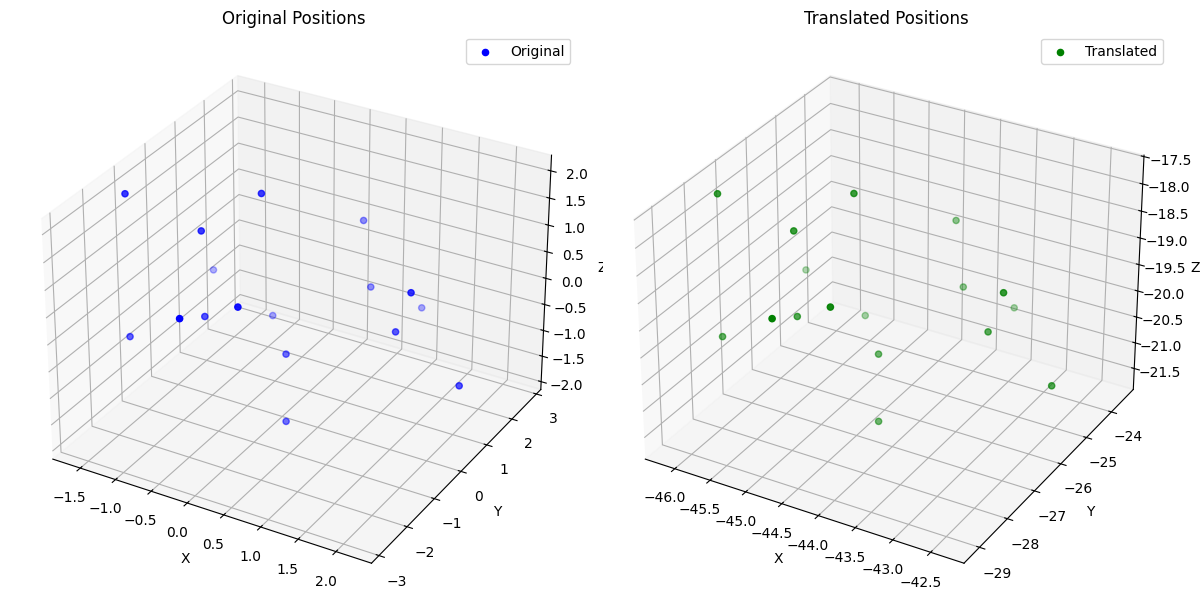
\includegraphics[width=0.9\linewidth]{Images_Ayoub/Invariance/Transformers/Translation.png}
  \caption{Visualization of the molecule before and after a random translation applied during the translation invariance test.}
  \label{fig:translation_invariance_visualization}
\end{figure}

\begin{lstlisting}[
  language={},
  basicstyle=\ttfamily\small,
  backgroundcolor=\color{lightgray},
  frame=single
]
=== Translation Invariance Test Report (23:58:44 2025-06-24) ===
Molecule ID: 6087

+-----------------------------------+---------------+
|              Metric               |     Value     |
+-----------------------------------+---------------+
| Predicted Energy (Not Translated) | -76.832260 eV |
|   Predicted Energy (Translated)   | -76.832260 eV |
|            True Energy            | -76.809608 eV |
|         Energy Difference         |  0.000000 eV  |
|         Invariance Check          |     PASS      |
+-----------------------------------+---------------+

Translation Vector:
+------+------------+
| Axis |   Value    |
+------+------------+
|  X   | -44.528400 |
|  Y   | -26.282589 |
|  Z   | -19.759033 |
+------+------------+

Atom Position Comparison (Part 1: Original Positions):
+----+-----------+-----------+-----------+
|    |   X_old   |   Y_old   |   Z_old   |
+----+-----------+-----------+-----------+
| 1  | 0.490875  | 1.959606  | -0.372477 |
| 2  | 1.310529  | 0.667022  | -0.309984 |
| 3  | 0.079384  | -0.057525 | -0.886156 |
| 4  | -0.62811  |  1.2522   | -1.038507 |
| 5  | -0.640845 | -1.064637 | 0.009023  |
| 6  | -0.72854  | -0.923804 | 1.490795  |
| 7  |  0.17009  | -1.90955  | 0.890594  |
| 8  | 0.916133  | 2.773638  | -0.981021 |
| 9  | 0.223377  |  2.38089  | 0.609945  |
| 10 | 1.621232  | 0.348187  | 0.687117  |
| 11 | 2.186306  | 0.649909  | -0.963593 |
| 12 | 0.265137  | -0.531613 | -1.871552 |
| 13 | -1.504396 | 1.302546  | -0.512791 |
| 14 | -1.491703 | -1.565303 | -0.474291 |
| 15 | -1.616365 | -1.302367 | 2.002271  |
| 16 | -0.237594 | -0.088436 | 1.991717  |
| 17 | -0.224412 | -2.84997  | 0.960382  |
+----+-----------+-----------+-----------+

Atom Position Comparison (Part 2: Translated Positions):
+----+------------+------------+------------+
|    |   X_new    |   Y_new    |   Z_new    |
+----+------------+------------+------------+
| 1  | -44.037525 | -24.322981 | -20.13151  |
| 2  | -43.217871 | -25.615565 | -20.069017 |
| 3  | -44.449016 | -26.340112 | -20.645189 |
| 4  | -45.15651  | -25.030387 | -20.79754  |
| 5  | -45.169245 | -27.347224 | -19.75001  |
| 6  | -45.25694  | -27.206391 | -18.268238 |
| 7  | -44.35831  | -28.192137 | -18.868439 |
| 8  | -43.612267 | -23.508949 | -20.740054 |
| 9  | -44.305023 | -23.901697 | -19.149088 |
| 10 | -42.907168 |  -25.9344  | -19.071916 |
| 11 | -42.342094 | -25.632678 | -20.722626 |
| 12 | -44.263263 |  -26.8142  | -21.630585 |
| 13 | -46.032796 | -24.980041 | -20.271824 |
| 14 | -46.020103 | -27.84789  | -20.233324 |
| 15 | -46.144765 | -27.584954 | -17.756762 |
| 16 | -44.765994 | -26.371023 | -17.767316 |
| 17 | -44.752812 | -29.132557 | -18.798651 |
+----+------------+------------+------------+

Atom Position Comparison (Part 3: Position Differences):
+----+----------+------------+------------+
|    |   dX     |    dY      |    dZ      |
+----+----------+------------+------------+
| 1  | -44.5284 | -26.282587 | -19.759033 |
| 2  | -44.5284 | -26.282587 | -19.759033 |
| 3  | -44.5284 | -26.282587 | -19.759033 |
| 4  | -44.5284 | -26.282587 | -19.759033 |
| 5  | -44.5284 | -26.282587 | -19.759033 |
| 6  | -44.5284 | -26.282587 | -19.759033 |
| 7  | -44.5284 | -26.282587 | -19.759033 |
| 8  | -44.5284 | -26.282587 | -19.759033 |
| 9  | -44.5284 | -26.282587 | -19.759033 |
| 10 | -44.5284 | -26.282587 | -19.759033 |
| 11 | -44.5284 | -26.282587 | -19.759033 |
| 12 | -44.5284 | -26.282587 | -19.759033 |
| 13 | -44.5284 | -26.282587 | -19.759033 |
| 14 | -44.5284 | -26.282587 | -19.759033 |
| 15 | -44.5284 | -26.282587 | -19.759033 |
| 16 | -44.5284 | -26.282587 | -19.759033 |
| 17 | -44.5284 | -26.282587 | -19.759033 |
+----+----------+------------+------------+
\end{lstlisting}



\subsubsection{Rotation Invariance Test Report}


To assess the rotation invariance of our model, we applied a random rotation defined by a given angle and axis to the atomic coordinates of a selected molecule. We then verified that the predicted energy remained unchanged and inspected how each atom's position transformed under this rotation.


\begin{figure}[H]
  \centering
  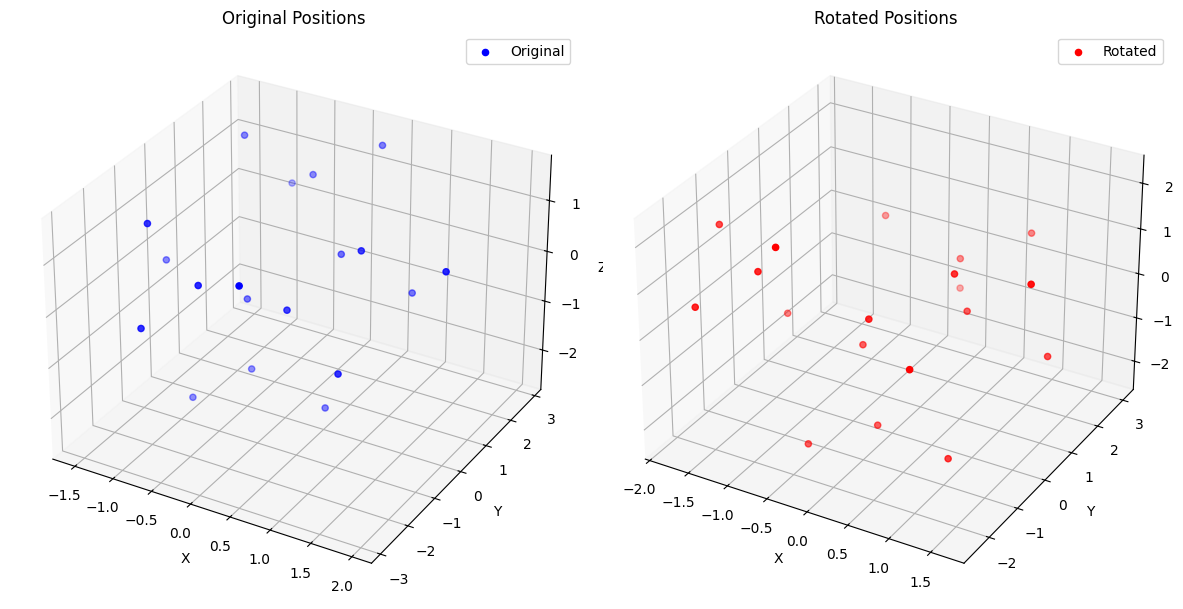
\includegraphics[width=0.9\linewidth]{Images_Ayoub/Invariance/Transformers/Rotation.png}
  \caption{Visualization of the molecule before and after a random rotation applied during the rotation invariance test.}
  \label{fig:rotation_invariance_visualization}
\end{figure}





\begin{lstlisting}[
  language={},
  basicstyle=\ttfamily\small,
  backgroundcolor=\color{lightgray},
  frame=single
]
=== Rotation Invariance Test Report (03:47:00 2025-06-29) ===
Molecule ID: 3548

+--------------------------------+---------------+
|             Metric             |     Value     |
+--------------------------------+---------------+
| Predicted Energy (Not Rotated) | -69.534927 eV |
|   Predicted Energy (Rotated)   | -69.534935 eV |
|          True Energy           | -69.579887 eV |
|       Energy Difference        |  0.000008 eV  |
|        Invariance Check        |     PASS      |
+--------------------------------+---------------+

Rotation Parameters:
+-------------------+----------------------------------+
|     Parameter     |              Value               |
+-------------------+----------------------------------+
| Point A (X, Y, Z) | (-0.680240, 0.382493, -0.664867) |
| Point B (X, Y, Z) | (-0.379383, 0.006690, 0.592881)  |
|  Axis (u, v, w)   | [0.300857, -0.375803, 1.257748]  |
|  Angle (radians)  |             4.646222             |
|  Angle (degrees)  |             266.21               |
+-------------------+----------------------------------+

Atom Pairwise Distances (Original, Rotated, Difference):
+-----------+--------------+--------------+-----------+
| Atom Pair | Old Distance | New Distance |   Diff    |
+-----------+--------------+--------------+-----------+
|    1-2    |   1.464718   |   1.464718   | -0.000000 |
|    1-3    |   2.476666   |   2.476666   |  0.000000 |
|    1-4    |   2.997632   |   2.997633   |  0.000001 |
|    1-5    |   4.343634   |   4.343635   |  0.000001 |
|    1-6    |   5.500458   |   5.500458   |  0.000000 |
|    1-7    |   1.016503   |   1.016502   | -0.000000 |
|    1-8    |   1.016903   |   1.016903   |  0.000000 |
|    1-9    |   2.141728   |   2.141728   |  0.000000 |
|   1-10    |   2.092613   |   2.092613   |  0.000000 |
|   1-11    |   2.741444   |   2.741444   | -0.000000 |
|   1-12    |   3.411400   |   3.411401   |  0.000001 |
|   1-13    |   3.350540   |   3.350542   |  0.000001 |
|   1-14    |   2.639691   |   2.639692   |  0.000000 |
|   1-15    |   6.532818   |   6.532818   |  0.000000 |
|    2-3    |   1.531452   |   1.531452   | -0.000000 |
|    2-4    |   2.550102   |   2.550102   |  0.000000 |
|    2-5    |   3.854393   |   3.854394   |  0.000000 |
|    2-6    |   4.998088   |   4.998088   | -0.000000 |
|    2-7    |   2.056355   |   2.056354   | -0.000001 |
|    2-8    |   2.057352   |   2.057352   | -0.000000 |
|    2-9    |   1.110689   |   1.110689   |  0.000000 |
|   2-10    |   1.099914   |   1.099914   |  0.000000 |
|   2-11    |   2.160242   |   2.160242   | -0.000001 |
|   2-12    |   2.155785   |   2.155786   |  0.000001 |
|   2-13    |   2.789115   |   2.789115   |  0.000001 |
|   2-14    |   2.773982   |   2.773981   | -0.000000 |
|   2-15    |   6.024486   |   6.024486   | -0.000000 |
|    3-4    |   1.536457   |   1.536457   |  0.000000 |
|    3-5    |   2.496576   |   2.496577   |  0.000000 |
|    3-6    |   3.557605   |   3.557605   | -0.000000 |
|    3-7    |   3.365947   |   3.365947   | -0.000000 |
|    3-8    |   2.683932   |   2.683933   |  0.000001 |
|    3-9    |   2.161960   |   2.161960   |  0.000000 |
|   3-10    |   2.168248   |   2.168247   | -0.000001 |
|   3-11    |   1.094869   |   1.094869   |  0.000000 |
|   3-12    |   1.094345   |   1.094345   |  0.000000 |
|   3-13    |   2.170651   |   2.170651   | -0.000000 |
|   3-14    |   2.165830   |   2.165829   | -0.000000 |
|   3-15    |   4.551731   |   4.551731   |  0.000000 |
|    4-5    |   1.463117   |   1.463117   |  0.000000 |
|    4-6    |   2.671470   |   2.671470   | -0.000001 |
|    4-7    |   3.929828   |   3.929828   |  0.000000 |
|    4-8    |   3.305116   |   3.305116   |  0.000000 |
|    4-9    |   3.497351   |   3.497352   |  0.000001 |
|   4-10    |   2.800982   |   2.800981   | -0.000000 |
|   4-11    |   2.160927   |   2.160928   |  0.000000 |
|   4-12    |   2.165203   |   2.165204   |  0.000001 |
|   4-13    |   1.098105   |   1.098106   |  0.000000 |
|   4-14    |   1.096899   |   1.096898   | -0.000000 |
|   4-15    |   3.733512   |   3.733512   | -0.000000 |
|    5-6    |   1.208353   |   1.208353   | -0.000001 |
|    5-7    |   5.319655   |   5.319655   |  0.000000 |
|    5-8    |   4.451129   |   4.451129   |  0.000001 |
|    5-9    |   4.652301   |   4.652301   |  0.000001 |
|   5-10    |   4.161105   |   4.161105   | -0.000000 |
|   5-11    |   2.729342   |   2.729342   |  0.000001 |
|   5-12    |   2.745279   |   2.745280   |  0.000000 |
|   5-13    |   2.096098   |   2.096098   |  0.000000 |
|   5-14    |   2.097593   |   2.097593   |  0.000000 |
|   5-15    |   2.270395   |   2.270394   | -0.000001 |
|    6-7    |   6.491732   |   6.491732   | -0.000000 |
|    6-8    |   5.511814   |   5.511814   | -0.000000 |
|    6-9    |   5.713261   |   5.713261   |  0.000000 |
|   6-10    |   5.325566   |   5.325565   | -0.000001 |
|   6-11    |   3.601385   |   3.601385   |  0.000000 |
|   6-12    |   3.621276   |   3.621276   | -0.000000 |
|   6-13    |   3.202369   |   3.202368   | -0.000000 |
|   6-14    |   3.204553   |   3.204553   | -0.000000 |
|   6-15    |   1.062042   |   1.062042   |  0.000000 |
|    7-8    |   1.651053   |   1.651053   |  0.000000 |
|    7-9    |   2.427278   |   2.427278   | -0.000000 |
|   7-10    |   2.391957   |   2.391956   | -0.000000 |
|   7-11    |   3.665340   |   3.665340   | -0.000001 |
|   7-12    |   4.187393   |   4.187393   |  0.000000 |
|   7-13    |   4.122169   |   4.122170   |  0.000001 |
|   7-14    |   3.564076   |   3.564075   | -0.000000 |
|   7-15    |   7.531528   |   7.531528   | -0.000000 |
|    8-9    |   2.469578   |   2.469579   |  0.000001 |
|   8-10    |   2.949858   |   2.949858   |  0.000000 |
|   8-11    |   2.522686   |   2.522686   | -0.000000 |
|   8-12    |   3.671317   |   3.671318   |  0.000001 |
|   8-13    |   3.923218   |   3.923219   |  0.000001 |
|   8-14    |   2.855042   |   2.855042   | -0.000000 |
|   8-15    |   6.487163   |   6.487163   |  0.000000 |
|   9-10    |   1.768109   |   1.768109   |  0.000000 |
|   9-11    |   2.497880   |   2.497879   | -0.000000 |
|   9-12    |   2.442635   |   2.442635   |  0.000000 |
|   9-13    |   3.779705   |   3.779706   |  0.000001 |
|   9-14    |   3.798965   |   3.798965   |  0.000000 |
|   9-15    |   6.687662   |   6.687663   |  0.000000 |
|  10-11    |   3.070779   |   3.070778   | -0.000001 |
|  10-12    |   2.501257   |   2.501257   | -0.000000 |
|  10-13    |   2.590000   |   2.590000   | -0.000000 |
|  10-14    |   3.125090   |   3.125090   | -0.000001 |
|  10-15    |   6.362715   |   6.362714   | -0.000001 |
|  11-12    |   1.754369   |   1.754369   |  0.000000 |
|  11-13    |   3.069997   |   3.069997   |  0.000000 |
|  11-14    |   2.517237   |   2.517237   | -0.000000 |
|  11-15    |   4.498767   |   4.498768   |  0.000000 |
|  12-13    |   2.518154   |   2.518154   |  0.000000 |
|  12-14    |   3.069016   |   3.069016   |  0.000000 |
|  12-15    |   4.520112   |   4.520112   | -0.000000 |
|  13-14    |   1.757575   |   1.757575   |  0.000001 |
|  13-15    |   4.220950   |   4.220949   | -0.000001 |
|  14-15    |   4.223501   |   4.223500   | -0.000000 |
+-----------+--------------+--------------+-----------+
\end{lstlisting}


% Outlining potential applications
\subsection{Training and Model Variants}

To evaluate the effectiveness of our Transformer-based approach for molecular energy prediction, we conducted three distinct training experiments:

\begin{enumerate}
    \item \textbf{Direct Use of Raw Positions}: In the first experiment, we trained the Transformer directly on the raw 3D atomic positions without any transformation. This approach violates key physical symmetries, such as translational, rotational, and permutational invariance, leading to a model that is sensitive to changes in molecular orientation or atom indexing.
    \item \textbf{Transformed Positions with Unsigned Angles}: In the second experiment, we applied the data transformation described in Section 2.2, computing invariant features (\( d_{CA} \), \( \theta_{CAF} \), \( \theta_{CAN} \)) but using unsigned angles. This ensured invariance under translation, rotation, and permutation. However, the lack of signed angles resulted in a non-bijective mapping between the computed features and the original atomic positions, potentially limiting the model's ability to fully reconstruct the molecular geometry.
    \item \textbf{Transformed Positions with Signed Angles}: In the final experiment, we used the complete transformation with signed angles, as detailed in Section 2.2. This approach ensures full invariance under translation, rotation, and permutation while maintaining a bijective relationship between the features and the molecular structure, making it theoretically optimal for the task.
\end{enumerate}

Among the three approaches, we focus our report and presentation exclusively on the most relevant variant: (V3) the model trained with transformed positions and signed angles. The other approaches, including the use of raw positions and the variant with unsigned angles, are not discussed further due to their lack of invariance to physical symmetries or their inferior theoretical foundation.


% Outlining potential applications
\subsubsection{Hyperparameters}

\subsubsubsection{V2 Model Architecture}


The V2 model leverages the data transformation described in Section 2.2, where each atom is represented by invariant features: the distance \( d_{CA} \) from the molecular centroid \( C \), and the unsigned angles \( \theta_{CAF} \) and \( \theta_{CAN} \). These features ensure invariance under translation, rotation, and permutation but lack the directional information provided by signed angles, which may limit the model’s ability to fully capture molecular geometry.

The Transformer architecture for V2 is configured as follows:

\begin{itemize}
    \item \textbf{Embedding Size}: The input embeddings, combining atom type and geometric features, have a dimensionality of \texttt{EMBEDDINGS\_SIZE = 1024}. This size balances expressive power with computational efficiency.
    \vspace{0.2cm}
    \item \textbf{Number of Attention Heads}: The multi-head attention mechanism uses \texttt{NB\_HEADS = 30}, allowing the model to capture diverse inter-atomic relationships.
    \vspace{0.2cm}
    \item \textbf{Query, Key, and Value Sizes}: Each attention head operates with \texttt{QUERY\_SIZE = 512}, \texttt{KEY\_SIZE = 512}, and \texttt{VALUE\_SIZE = 512}, ensuring sufficient capacity for attention computations.
    \vspace{0.2cm}
    \item \textbf{Attention Blocks}: The model includes \texttt{NB\_ATTENTION\_BLOCKS = 1}, focusing on a single layer of attention to reduce complexity while maintaining effective interaction modeling.
    \vspace{0.2cm}
    \item \textbf{MLP for Attention Weights (WQ, WK, WV)}: The multilayer perceptron (MLP) used to compute attention weights (for query, key, and value projections) consists of \texttt{NB\_HIDDEN\_LAYERS\_MLP\_ATTENTION\_WQ\_WK\_WV = 5} layers, with sizes \texttt{[32, 64, 128, 256, 512]} and activation function \texttt{ACTIVATION\_NAME\_MLP\_ATTENTION\_WQ\_WK\_WV = `PReLU'}. This configuration allows gradual feature expansion.
    \vspace{0.2cm}
    \item \textbf{MLP for Attention Output (WO)}: The MLP for the attention output projection has \texttt{NB\_HIDDEN\_LAYERS\_MLP\_ATTENTION\_WO = 5} layers, with sizes \texttt{[64, 128, 256, 512, 1024]} and activation \texttt{ACTIVATION\_NAME\_MLP\_ATTENTION\_WO = `PReLU'}, aligning the output with the embedding size.
    \vspace{0.2cm}
    \item \textbf{Output MLP}: The final MLP, which produces the molecular energy prediction, comprises \texttt{NB\_HIDDEN\_LAYERS\_MLP\_OUTPUT = 5} layers with sizes \texttt{[512, 256, 128, 64, 32]}, an output size of \texttt{OUTPUT\_SIZE = 1}, and activation \texttt{ACTIVATION\_NAME\_OUTPUT = `PReLU'}. This architecture progressively refines the CLS token representation into a single scalar prediction.
\end{itemize}
\vspace{0.2cm}

\subsubsubsection{Optimization parameters}
The training is performed using the Adam optimizer, which is well-suited for handling sparse gradients and adaptive learning rates. The learning rate is set to \(3 \times 10^{-5}\), and the computations are executed on a GPU with 4GB of memory to accelerate the training process.

\subsubsubsection{Training Schedule}
In practice, an initial training of the model is generally performed for 450 epochs using the hyperparameters described above. This phase allows the model to learn a robust representation of molecules from the transformed data. \newline

The dataset was split into 80\% for training and 20\% for testing, ensuring that model evaluation is performed on unseen molecules. \newline

The loss function used for training is the Mean Squared Error (MSE), which is standard for regression tasks such as molecular energy prediction. \newline

For the V3 model (using signed angles), it is possible to further improve performance by continuing the training for an additional 100 epochs, but with a reduced learning rate of \(3 \times 10^{-6}\). This fine-tuning step helps to enhance final convergence and optimize the accuracy of molecular energy prediction.

\subsubsubsection{Loss Evolution}
The figure below shows the evolution of the loss function during training, plotted on a logarithmic scale. The two images above display the loss per epoch, while the image below presents the loss per batch. This visualization allows for a detailed analysis of the model's convergence behavior at both the epoch and batch levels.
\begin{figure}[H]
  \centering
  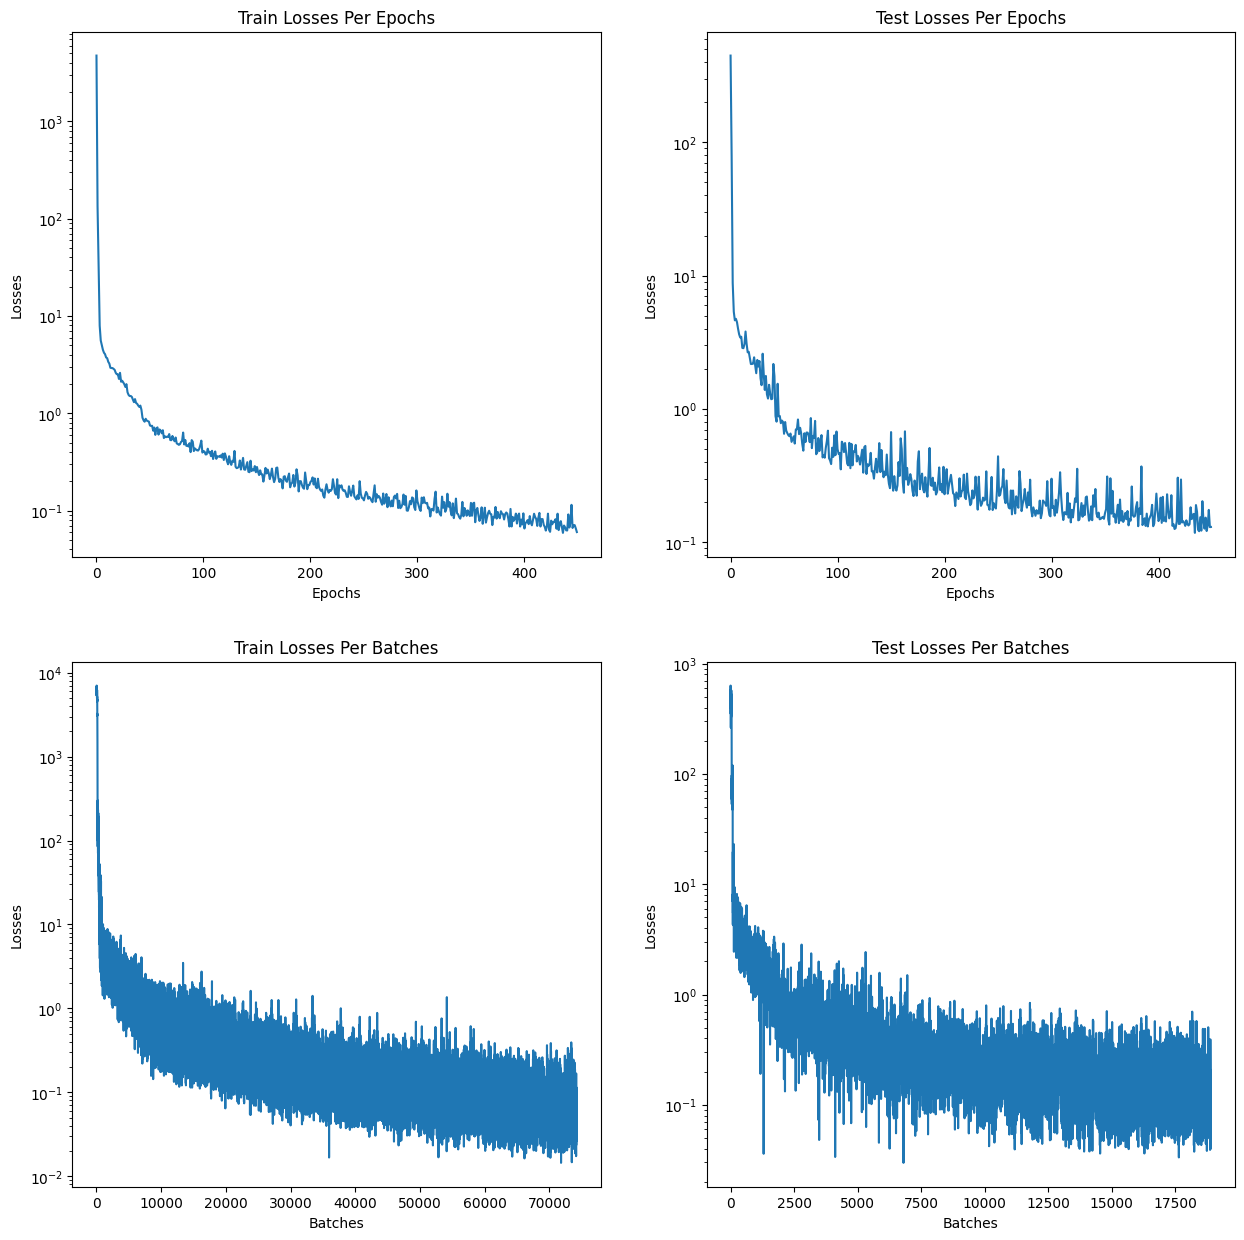
\includegraphics[width=0.9\linewidth]{Images_Ayoub/Training/Transformers/V3/Losses/First_450_Epochs/Loss.png}
  \caption{Evolution of the loss function during training of the Transformer model for molecular energy prediction (logarithmic scale).}
  \label{fig:transformer_loss_evolution}
\end{figure}



The provided graphs illustrate the \textbf{training} and \textbf{test losses} over \textbf{epochs} and \textbf{batches}, highlighting the model's convergence behavior. The top-left graph shows \textbf{train losses} per \textbf{epoch}, dropping sharply from approximately \( \mathbf{10^3} \) to \( \mathbf{10^0} \) within the first \textbf{50 epochs}, followed by a gradual stabilization around \( \mathbf{10^{-1}} \) by \textbf{epoch 400}, indicating effective learning. The top-right graph depicts \textbf{test losses} per \textbf{epoch}, decreasing from \( \mathbf{10^3} \) to \( \mathbf{10^{-1}} \) with fluctuations peaking around \( \mathbf{10^0} \) after \textbf{200 epochs}, suggesting some variance in generalization. The bottom-left graph, representing \textbf{train losses} per \textbf{batch}, shows a detailed decline from \( \mathbf{10^4} \) to \( \mathbf{10^{-1}} \) over \textbf{70,000 batches}, with significant noise reflecting the iterative optimization process. Lastly, the bottom-right graph of \textbf{test losses} per \textbf{batch} mirrors this trend, dropping from \( \mathbf{10^4} \) to \( \mathbf{10^{-1}} \) with oscillations reaching up to \( \mathbf{10^0} \) around \textbf{15,000 batches}, possibly indicating overfitting or data variability. Overall, these trends suggest a robust \textbf{training process} with room for further tuning to enhance model generalization. \newline

These results demonstrate that the model is able to learn the molecular energy prediction task effectively, without any apparent signs of overfitting: the test loss follows the same trend as the training loss, and no significant divergence is observed between the two curves. This indicates a good generalization capability of the model on molecules not seen during training.

\subsubsubsection{Kaggle Result}

The model was evaluated on the Kaggle platform, where it achieved a score of 0.311 on the leaderboard. This score reflects the model's performance in predicting molecular energies based on the test dataset provided by Kaggle. The result indicates that the Transformer-based approach, particularly with the use of transformed positions and signed angles, is effective for this task, achieving a competitive score in the context of molecular property prediction challenges.



\subsection{CLS Embeddings Visualisation}

In order to visualize the embeddings of the CLS token, we applied a dimensionality reduction technique, specifically t-SNE (t-distributed Stochastic Neighbor Embedding), to project the high-dimensional CLS embeddings into a 2D space. This allows us to observe how different molecules are distributed based on their learned representations.

\begin{figure}[H]
  \centering
  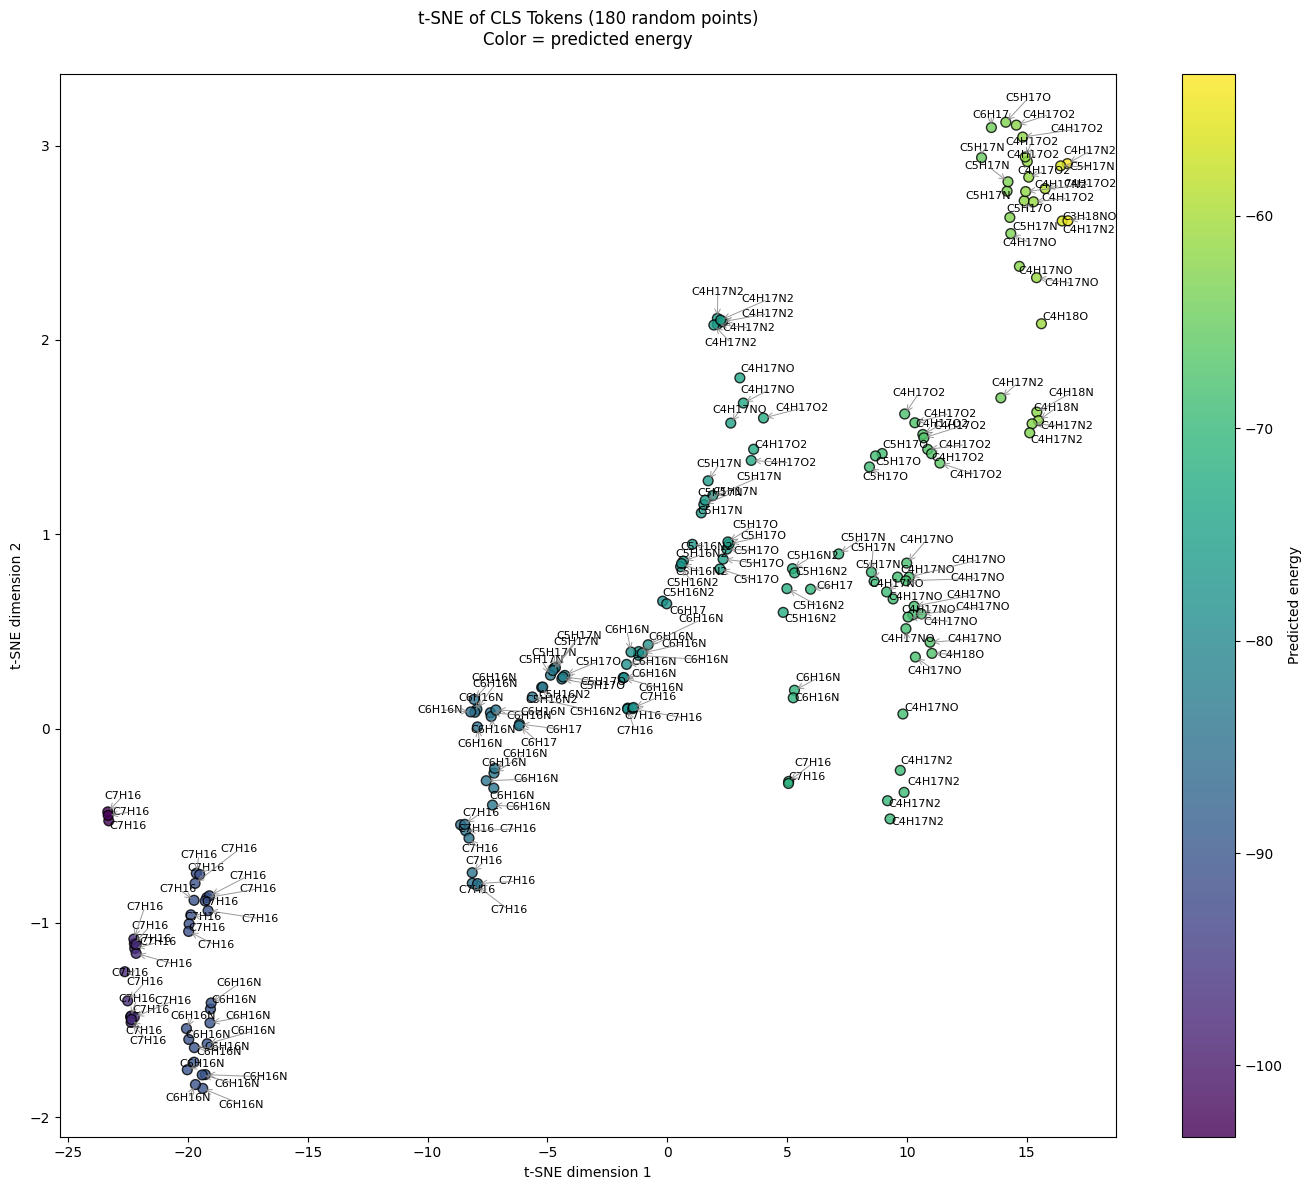
\includegraphics[width=0.9\linewidth]{Images_Ayoub/Training/Transformers/V3/Visualisation_CLS_TOKENS/Image.png}
  \caption{Visualization of CLS token embeddings after dimensionality reduction with t-SNE.}
  \label{fig:cls_embeddings_tsne}
\end{figure}

As shown in Figure~\ref{fig:cls_embeddings_tsne}, the two-dimensional t-SNE projection of the CLS token embeddings highlights meaningful structure in the learned representation space. Molecules with similar predicted energies tend to cluster together, suggesting that the model has captured relevant chemical and energetic features in the high-dimensional embedding space.

\section{Further Work and approaches}

\subsubsection{Path-Augmented Graph Transformer Network (PAGTN)}

As a promising future direction, we propose exploring the \textbf{Path-Augmented Graph Transformer Network (PAGTN)} for enhanced molecular energy prediction. PAGTN combines the strengths of graph neural networks and transformers while addressing the limitations of local message passing in standard Graph Convolutional Networks (GCNs). Specifically, it incorporates \emph{path features} to model long-range dependencies in molecular graphs, as originally introduced by Chen et al.\ in Path-Augmented Graph Transformer Network. \newline

In the PAGTN framework, atoms and bonds are encoded as nodes and edges of a molecular graph. The model uses shortest-path information between pairs of atoms to build three types of path features: \newline
\begin{itemize}
    \item \textbf{Edge features:} concatenation of individual bond features (e.g., bond type, conjugacy, ring membership) along the path.
    \vspace{0.2cm}
    \item \textbf{Distance encoding:} one-hot representation of the shortest-path distance between nodes, truncated at a maximum value $d$.
    \vspace{0.2cm}
    \item \textbf{Ring membership:} one-hot encoding indicating whether the two atoms belong to the same ring (including special encodings for 5- or 6-membered aromatic rings).
    \vspace{0.2cm}
  \end{itemize}

These path features are incorporated directly into the transformer’s attention mechanism, allowing each node to attend to all others in the graph globally, with attention weights modulated by structural relationships. Compared to GCNs, which require many layers to propagate information across distant nodes, PAGTN can learn such dependencies in fewer layers. \newline

The architecture consists of multiple global self-attention layers followed by feed-forward layers, with layer normalization and residual connections. After node embeddings are updated, a permutation-invariant pooling is used to generate a global molecular representation, which is passed through a multilayer perceptron to predict the molecular property (e.g., energy). \newline

PAGTN offers several advantages:
\vspace{0.2cm}
\begin{itemize}
  \item \textbf{Enhanced expressivity:} meilleure représentation des sous-structures importantes (par exemple, cycles, chaînes) via la modélisation au niveau des chemins.
  \vspace{0.2cm}
  \item \textbf{Long-range modeling:} capture efficace des interactions non locales sans empilement profond de couches.
  \vspace{0.2cm}
  \item \textbf{Physical consistency:} meilleure préservation de l'invariance par permutation et potentiel pour des extensions géométriques.
\end{itemize}
\vspace{0.2cm}




\section*{Conclusion}

In this project, we explored two complementary approaches to the challenging task of molecular energy prediction: a wavelet-based method leveraging 3D scattering transforms, and a Transformer-based model enriched with geometric invariants. Both methods were designed to respect the fundamental symmetries of molecular physics—namely translation, rotation, and permutation invariance—ensuring physically consistent predictions. \newline

The wavelet scattering approach demonstrated how local and global geometric features can be extracted in a mathematically rigorous way, yielding interpretable representations well-suited for regression. On the other hand, the Transformer-based architecture, empowered by a tailored data transformation pipeline, showed promising flexibility and scalability, while preserving critical invariance properties. \newline

Our experimental results, validated on the QM7-X dataset, confirm that respecting physical symmetries not only improves predictive accuracy but also contributes to model robustness. Future work will aim to combine the strengths of both methods, and explore more expressive architectures such as Path-Augmented Graph Transformers (PAGTNs) to further enhance performance and interpretability in quantum chemistry regression tasks. \newline



\end{document}